\documentclass[12pt]{report}
\usepackage{graphicx}
\usepackage{blindtext}
\usepackage{caption}
\usepackage{subcaption}
\usepackage{titlesec}
\usepackage{lipsum}
\usepackage{tabu}
\usepackage[inkscapeformat=png]{svg}
\usepackage[polish]{babel}
\usepackage[T1]{fontenc}
\usepackage[utf8]{inputenc}
\usepackage{csquotes}
\usepackage[backend=biber]{biblatex}
\usepackage[a4paper,width=150mm,top=10mm,bottom=25mm,bindingoffset=6mm]{geometry}

\addbibresource{bibliography.bib}
\graphicspath{ {images/} }
\linespread{1.5}
\title{ZodiaCal}
\author{Elżbieta Kołcz}
\date{Day Month Year}

\titleformat{\chapter}{\bfseries\Huge}{{\Huge\thechapter}}{1em}{}
\renewcommand*\contentsname{Spis treści}
\renewcommand{\listfigurename}{Spis rysunków}
\renewcommand{\listtablename}{Spis tabel}

\begin{document}
% !TeX spellcheck = pl
\begin{titlepage}
    \begin{center}
        \vspace*{1cm}
        
        \Huge
        \textbf{ZodiaCal}
        
        \vspace{0.5cm}
        \LARGE
        Zintegrowany Kalendarz Osobisty z Planerem Pielęgnacji Cery

        \vspace{5cm}

        
        \textbf{Elżbieta Kołcz 81640}


        \vspace{0.5cm}

        \Large
        Uniwersytet WSB Merito we Wrocławiu\\
        Wydział Finansów i Zarządzania\\
        Kierunek: Informatyka inżynierska\\
        2025
        
        \vfill
        Opiekun naukowy\\
        mgr inż. Stanisław Lota

        
        \vspace{0.8cm}
    \end{center}
\end{titlepage}

\tableofcontents

\listoffigures

\chapter{Wprowadzenie}
W obecnych warunkach społeczno-ekonomicznych wielu studentów podczas toku swojego nauczania podejmuję pracę dorywczą. Zarządzanie nawarstwiającymi się wydarzenia typu egzaminy, projekty zaliczeniowe, spotkania biznesowe, czy po prostu wyjścia ze znajomymi mogą być dla wielu osób przytłaczające. Do tego wszystkiego dochodzi moda na prowadzenie zdrowego trybu życia, które niejako wiąże się z dbaniem o cerę poprzez skomplikowaną, rozbudowaną pielęgnację z użyciem różnych produktów. Wśród młodych dorosłych zanika potrzeba prowadzenia klasycznego, papierowego kalendarza. Wszystko odbywa się z wykorzystaniem aplikacji mobilnych, ponieważ jest to wygodne rozwiązanie, telefon jest zawsze w zasięgu ręki, a powiadomienia o nadchodzących wydarzeniach wielokrotnie były nieocenionym wsparciem.

Stworzona na potrzeby pracy dyplomowej aplikacja star się ułatwić użytkownikom efektywną organizację wielu wydarzeń, a także zapewnienia wsparcia w codziennej pielęgnacji. Opracowane narzędzie posiada opcję automatycznego uzupełniania pól w kalendarzu z rozróżnieniem na kategorie praca / studia co w przypadku cyklicznych wydarzeń znacząco oszczędza czas i eliminuje konieczność wykonywania powtarzalnych czynności przez użytkownika. Dodatkowo aplikacja ma wbudowaną funkcję analizy pielęgnacji cery umożliwiającą monitorowanie w jakim stopniu pielęgnacja w danym miesiącu była nawilżająca, złuszczająca czy regeneracyjna. Co więcej użytkownicy mają dostęp do codziennych horoskopów dostosowanych do ich znaków zodiaku. Jeśli użytkownik nie zna bądź nie wie w jaki sposób określić swój znak zodiaku, aplikacja po utworzeniu konta i kliknięcia w zakładkę Horoscope pyta o dzień i miesiąc urodzenia, a następnie automatycznie przydziela znak zodiaku na podstawie podanej daty.

Celem pracy inżynierskiej jest zapewnienie wsparcia dla ambitnych młodych dorosłych, którzy dążą do maksymalnego wykorzystania życia. Co prawda jest wiele aplikacji o charakterze kalendarza dostępnych na rynku, jednak większość z nich jest przeznaczona dla innego użytkownika końcowego, tzw. na przykład dla zespołów pracujących w firmie. Dodatkowo
w tej chwili rynek rozdziela kalendarz osobisty i dzienniczek pielęgnacji na dwie różne aplikację, co prowadzi do tego, że użytkownik nie tylko musi uzupełniać pola w dwóch różnych miejscach, uczyć się dwóch różnych interfejsów, ale również przekazywać swoje dane do dwóch różnych serwisów.



\chapter{Analiza i badania rynku}
\phantom{Th}
Analiza biznesowa jest nieodłącznym elementem procesu planowania i podejmowania decyzji, które umożliwiającym lepsze zrozumienie kontekstu strategicznego, w jakim realizowany jest projekty. Polega ona na przygotowaniu zestawu zadań i technik, które stanowią łącznik między interesariuszami mając na celu zrozumienie w jaki sposób organizacje funkcjonują w dążeniu do osiągnięcia swoich celów. Ponadto, analiza biznesowa definiuje możliwości, których organizacja potrzebuje, aby skutecznie dostarczać produkty i usługi zewnętrznym interesariuszom \cite{businessanalysis}. Jest to kluczowy etap, pozwalający na identyfikację elementów, które mogą przyczynić się do sukcesu organizacji w zmieniającym się otoczeniu rynkowym.

\section{Analiza konkurencyjnych rozwiązań}

\phantom{Th}Na rynku znajduje się wiele narzędzi do organizacji czasu, ale \textbf{kalendarz Google} pozostaje niekwestionowanym liderem.
Jest to profesjonalne i przede wszystkim darmowe, domyślne narzędzie na większości urządzeń z systemem Android.
Według raportu stworzonego przez zespół pracujący dla DataReportal, w Polsce na rok 2023, aż 87\% użytkowników posiada
telefon właśnie z tym systemem
\cite{datareportal}. Aplikacja ta stanowi nieodłączny element funkcjonowania firm, zwłaszcza tych początkujących,
ale nie tylko. Ułatwia harmonogramowanie spotkań, śledzenie projektów i pozwala na zachowanie kontroli nad terminami.
Dużym atutem kalendarza Google jest rozdzielenie zadań i wydarzeń na osobne elementy (Rysunek \ref{fig:googleCalendar}).

Jest to narzędzie umożliwiające precyzyjne określenie wszelkich informacji odnośnie danego wydarzenia.
Nie da się kwestionować, że możliwości jakie daje nam aplikacja są niepotrzebne,
jednakże z punktu widzenia użytkownika końcowego ZodiaCal funkcje takie jak lokalizacja wydarzenia,
link do rozmowy wideo czy określanie trwania każdego wydarzenia od do jest zbędne.
W ZodiaCal istotne jest sprawne dodawanie wydarzeń do kalendarza, bez konieczności przeglądania dodatkowych opcji.

Dobrą alternatywą dla kalendarza Google jest \textbf{Proton Calendar} (Rys. \ref{fig:protonCalendar}).
Jest to również zaawansowana aplikacja do monitorowania wydarzeń, z tą różnicą,
iż proton specjalizuje się w zapewnianiu jeszcze większej prywatności i bezpieczeństwa użytkowników.
Z tym, że nie rozróżnia wydarzeń od zadań. Proton to firma oferująca usługi związane
z prywatnością online, w tym bezpiecznymi skrzynkami e-mail i kalendarzami.

Bardzo ciekawym i minimalistycznym rozwiązaniem jest aplikacja \textbf{135 To Do List} która poprzez swój estetyczny
i prosty interfejs ułatwia użytkownikom ustalanie priorytetów zadań na konkretny dzień.
Posiada możliwość zmiany kolejności wpisanych już wcześniej zadań oraz widok całego miesiąca.
Niestety nie ma opcji dodawania cyklicznych wydarzeń. ZodiaCal przyświeca niemalże ta sama minimalistyczna
idea tworzenia interfejsu, jednak wprowadza rozbudowane funkcje, takie jak codzienny horoskop i osobisty dziennik pielęgnacji (Rys. \ref{fig:ToDoList}).

\begin{figure}[t]
	\begin{minipage}{0.4\textwidth}
		\centering
		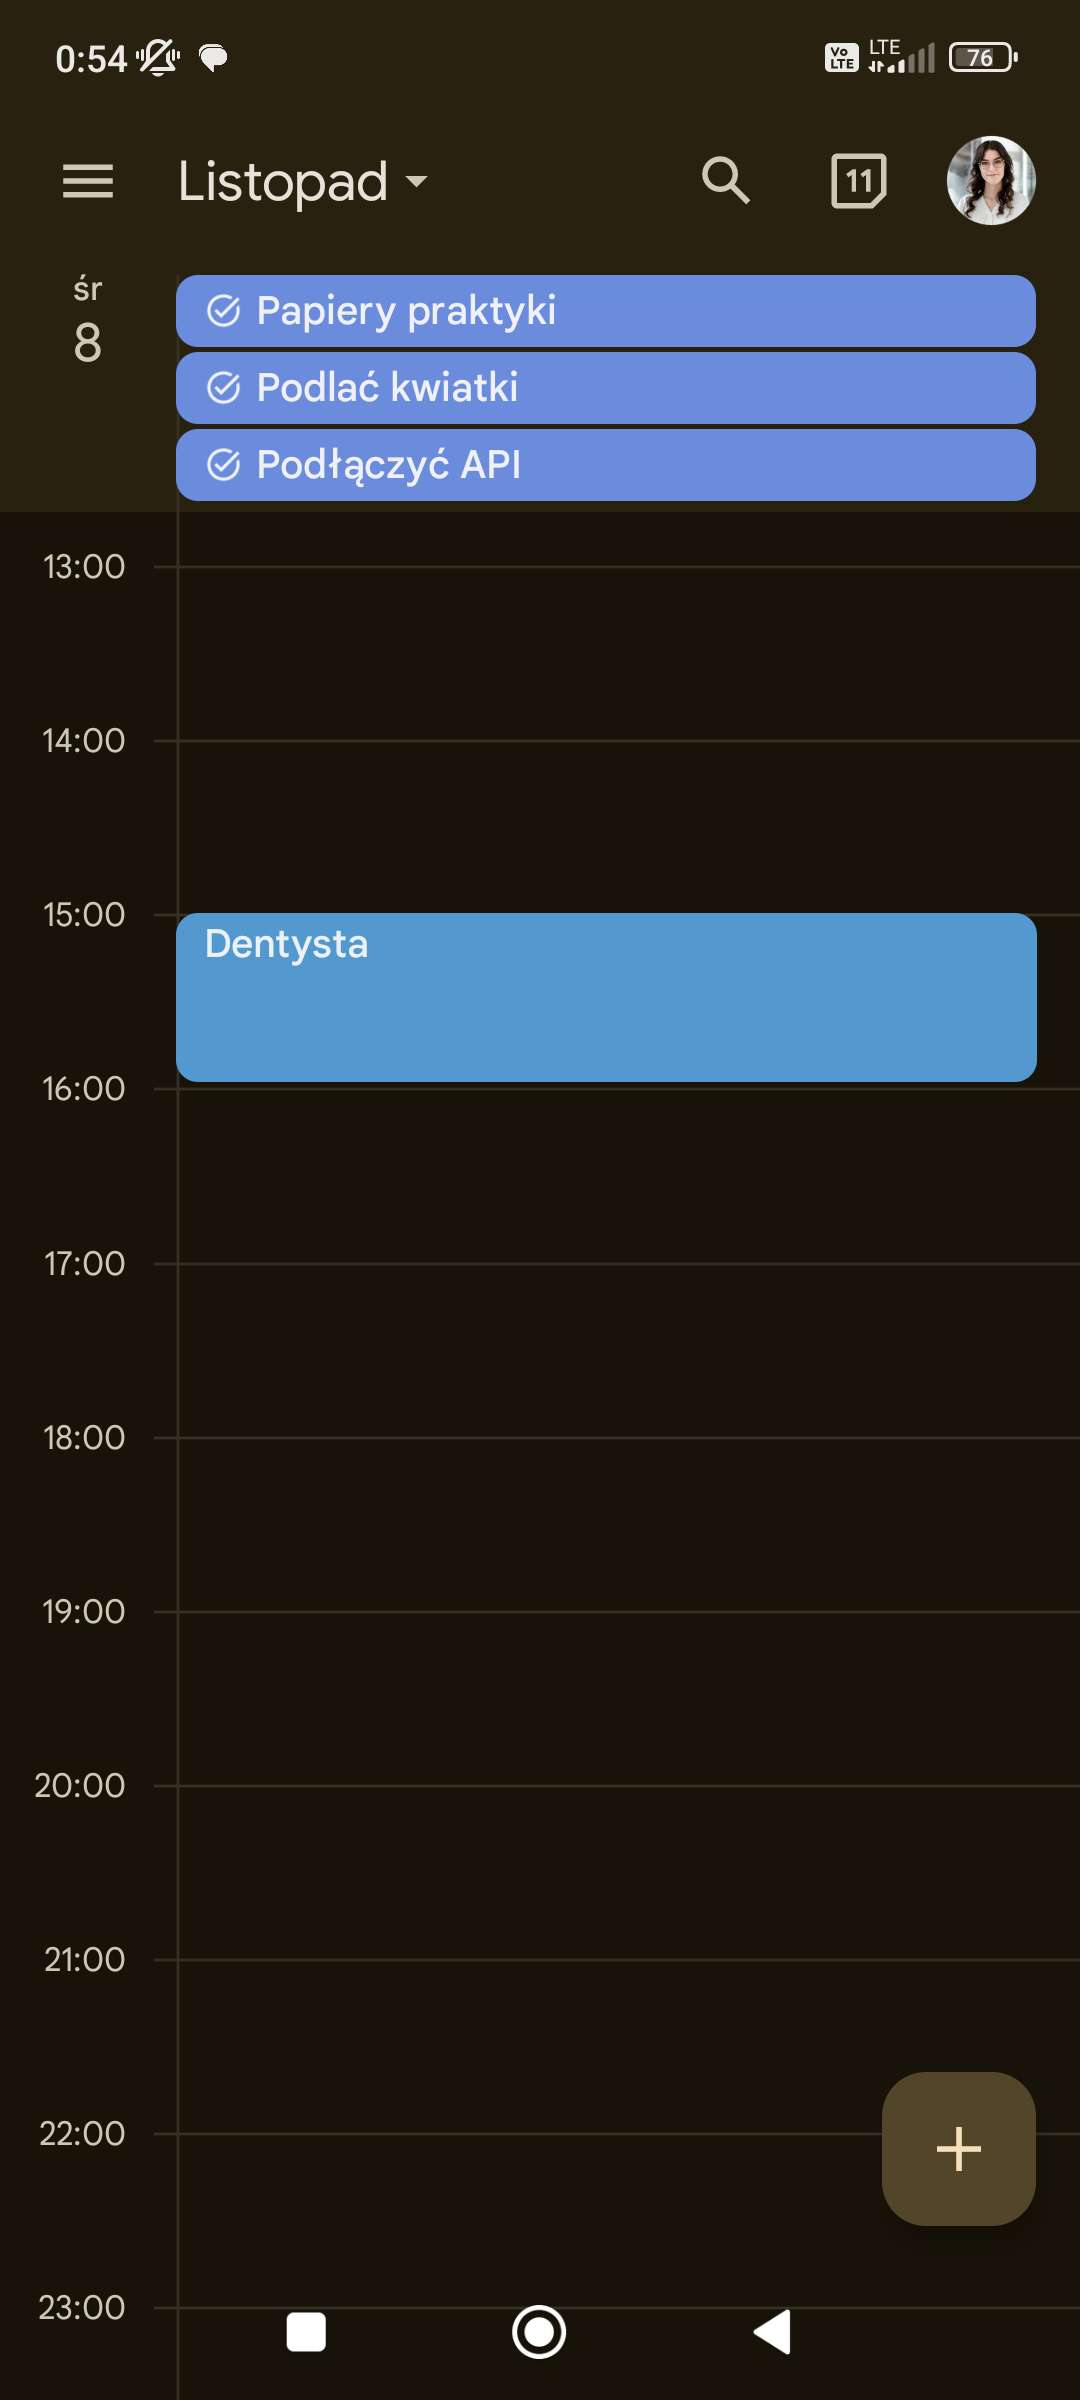
\includegraphics[height=13cm, keepaspectratio]{images/analiza/googleCalendar}
		\caption{Widok konkretnego dnia w kalendarzu Google}
		\label{fig:googleCalendar}
	\end{minipage}
	\hfill
	\begin{minipage}{0.4\textwidth}
		\centering
		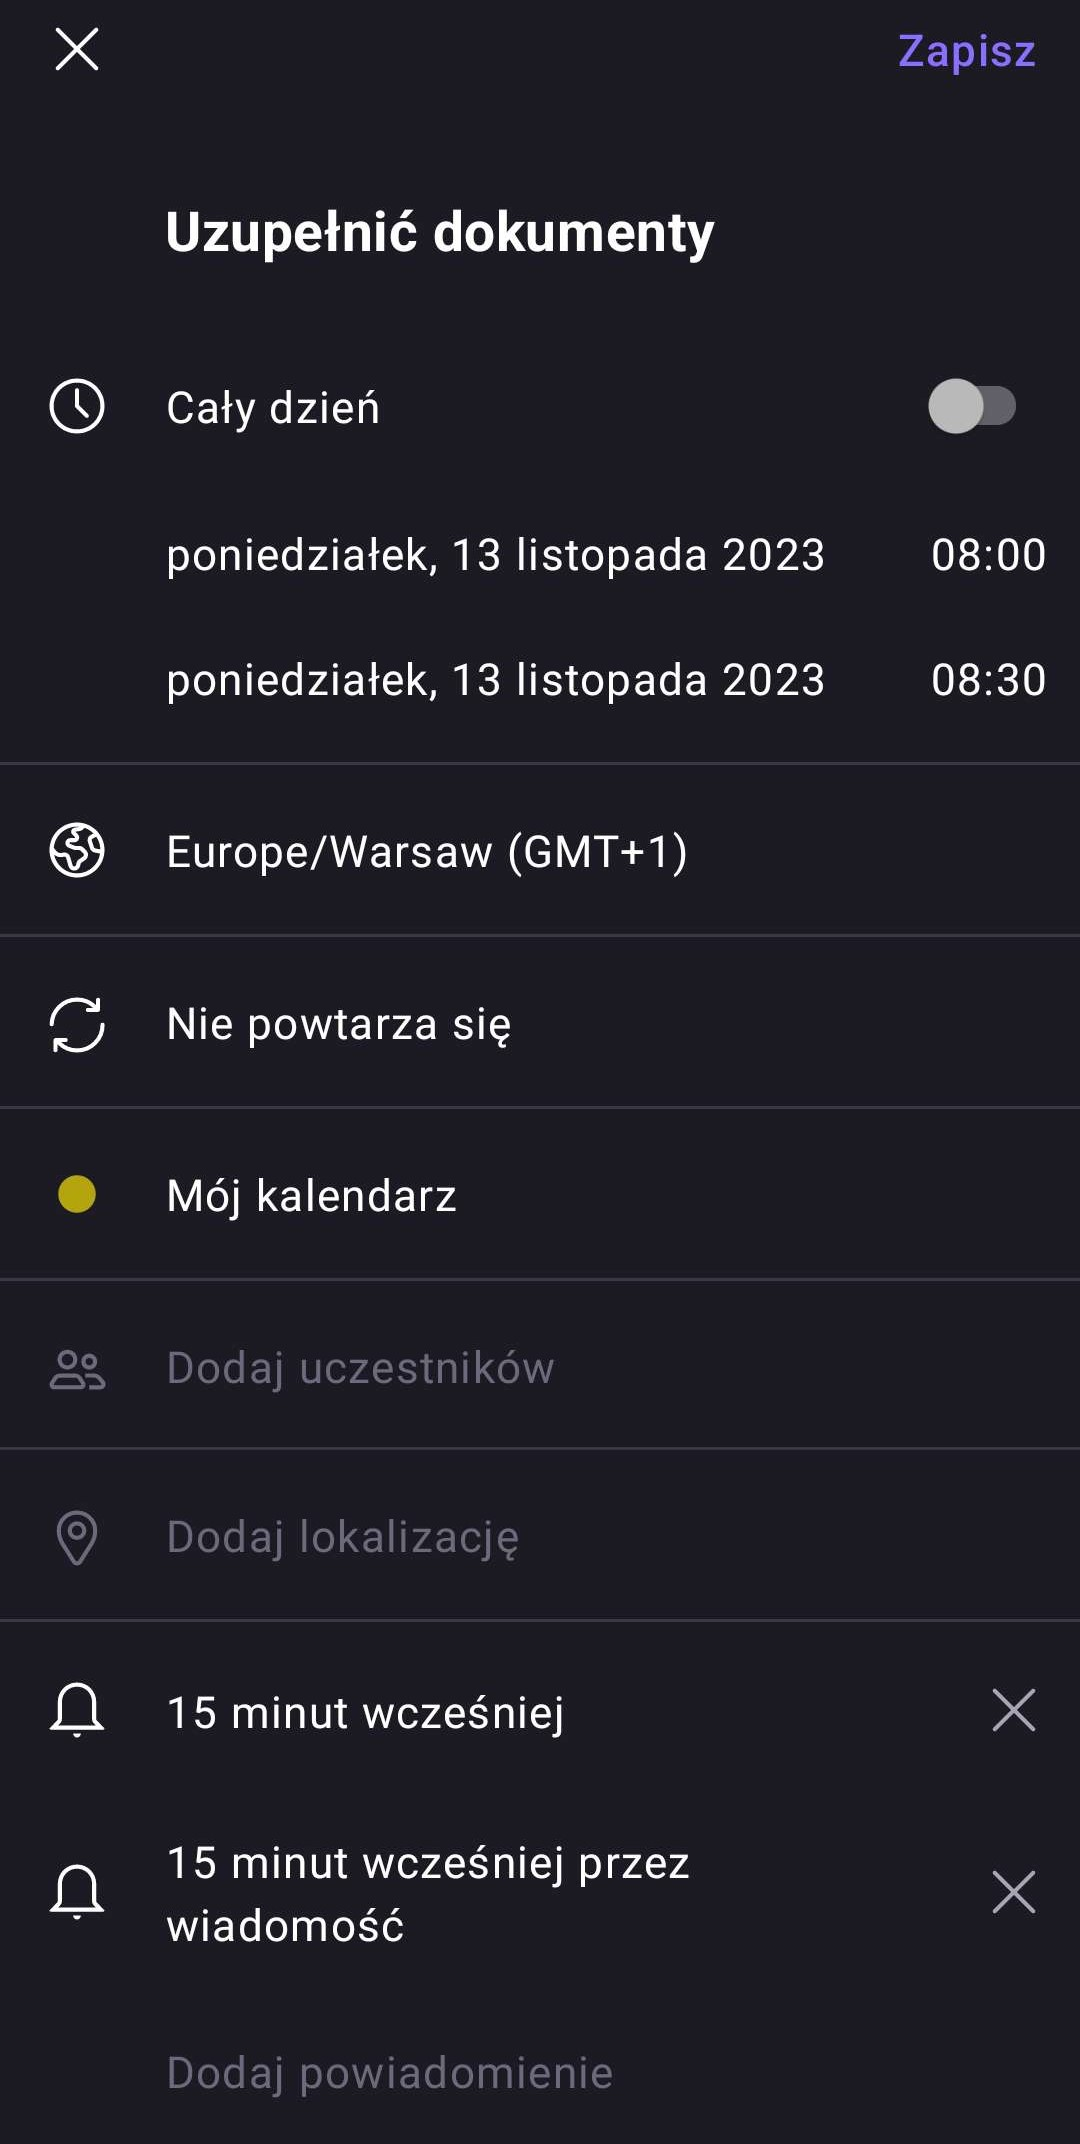
\includegraphics[height=13cm, keepaspectratio]{images/analiza/protonCalendar}
		\caption{Widok tworzenia wydarzenia w kalendarzu Proton}
		\label{fig:protonCalendar}
	\end{minipage}
\end{figure}

\newpage
\textbf{FeelingMySkin} to bardzo rozbudowane narzędzie do precyzyjnego określenia pielęgnacji cery i nie tylko.
Korzystając z niej użytkownik może układać plany pielęgnacyjne z wykorzystaniem konkretnych produktów,
których używa na co dzień, monitorować zmiany skórne, czy chociażby śledzić daty przydatności produktów.
To z pewnością przydatna aplikacja, jednakże wymaga czasu, aby opanować wszystkie możliwe funkcje.
Interfejs strony głównej jest bardzo przeładowany informacjami, co utrudnia korzystanie z aplikacji w sposób efektywny (Rys. \ref{fig:feelingMySkin}).

\begin{figure}[ht]
  \begin{minipage}{0.4\textwidth}
    \centering
    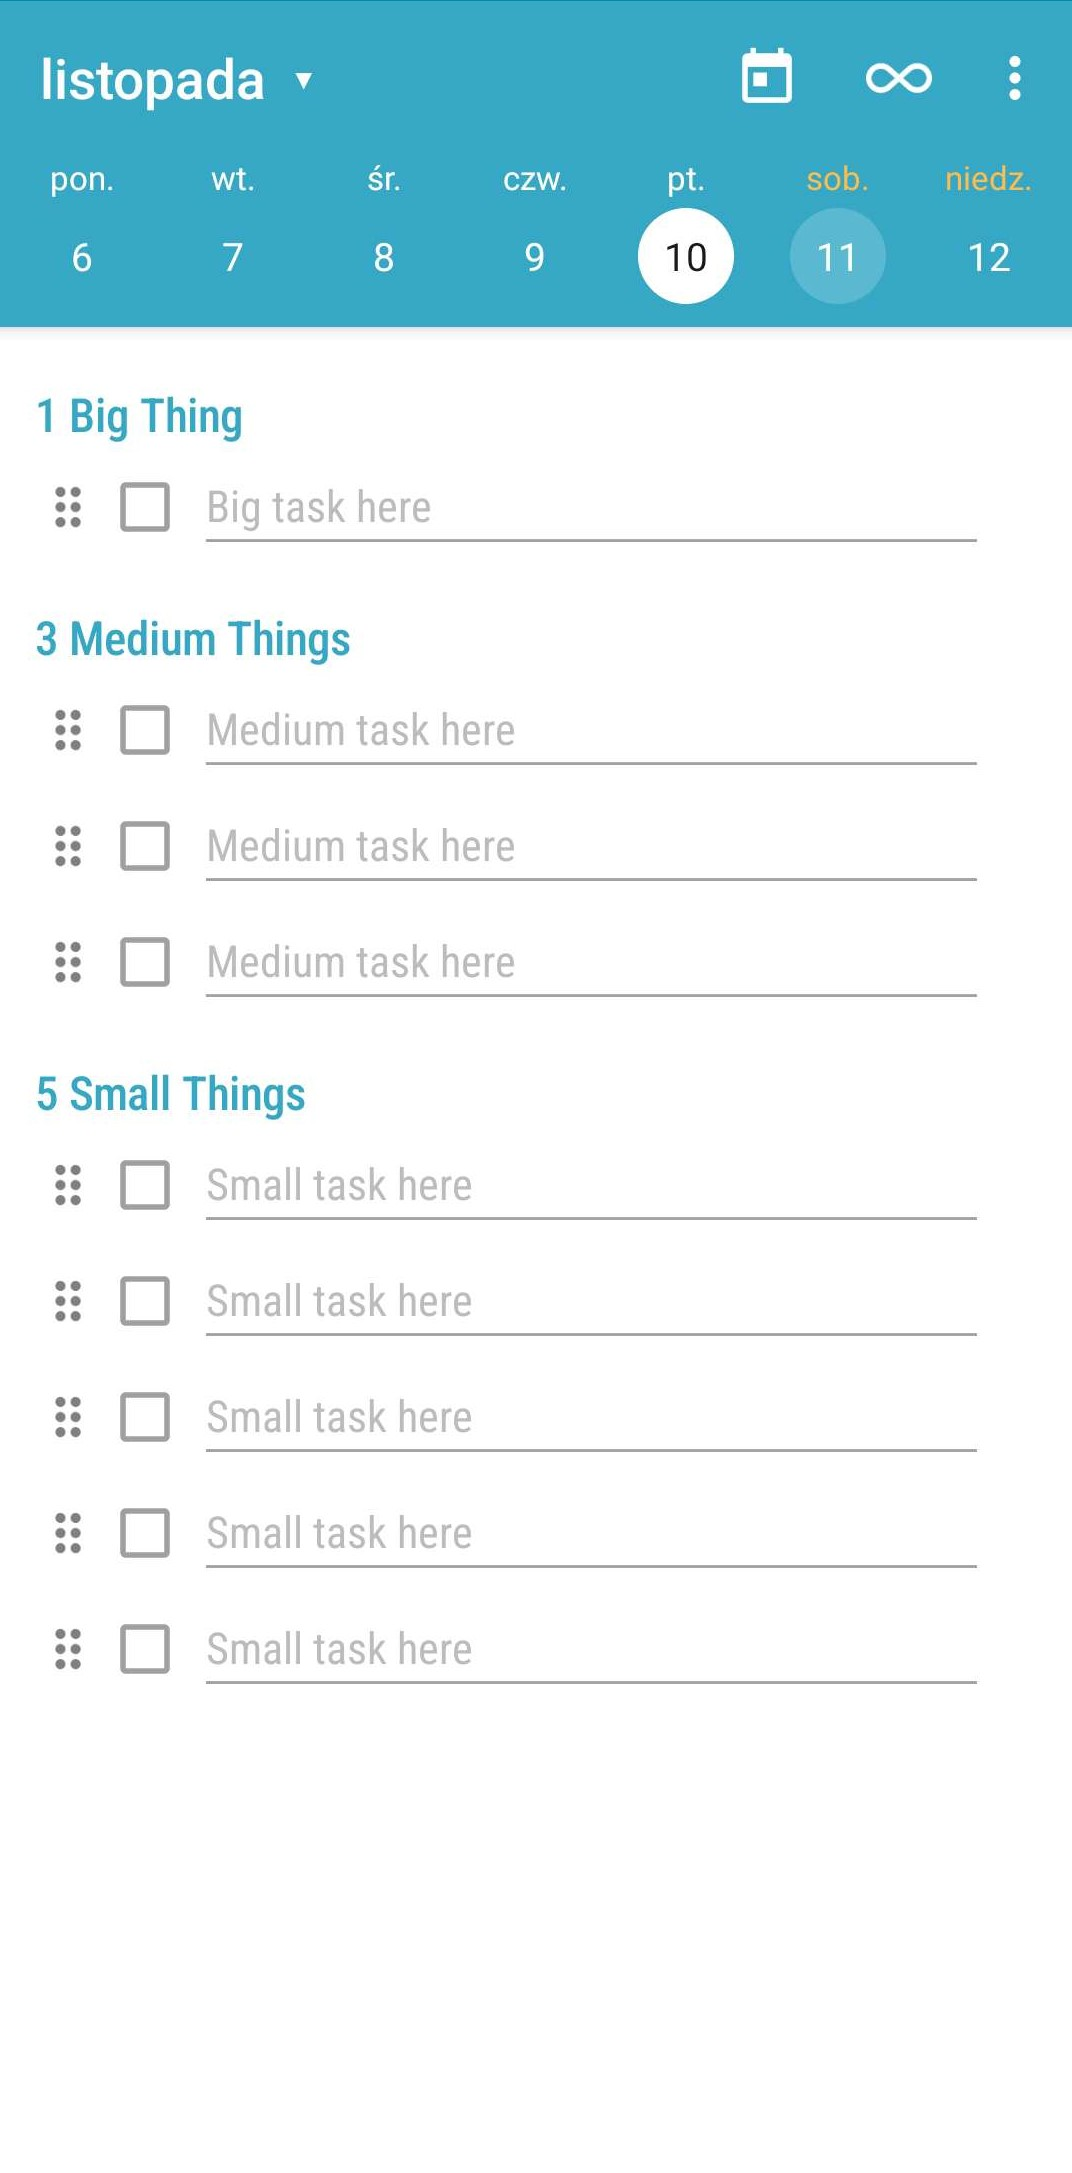
\includegraphics[height=13cm, keepaspectratio]{images/analiza/135ToDoList}
    \caption{Ekran główny aplikacji 135 To Do List}
    \label{fig:ToDoList}
  \end{minipage}
  \hfill
  \begin{minipage}{0.4\textwidth}
    \centering
    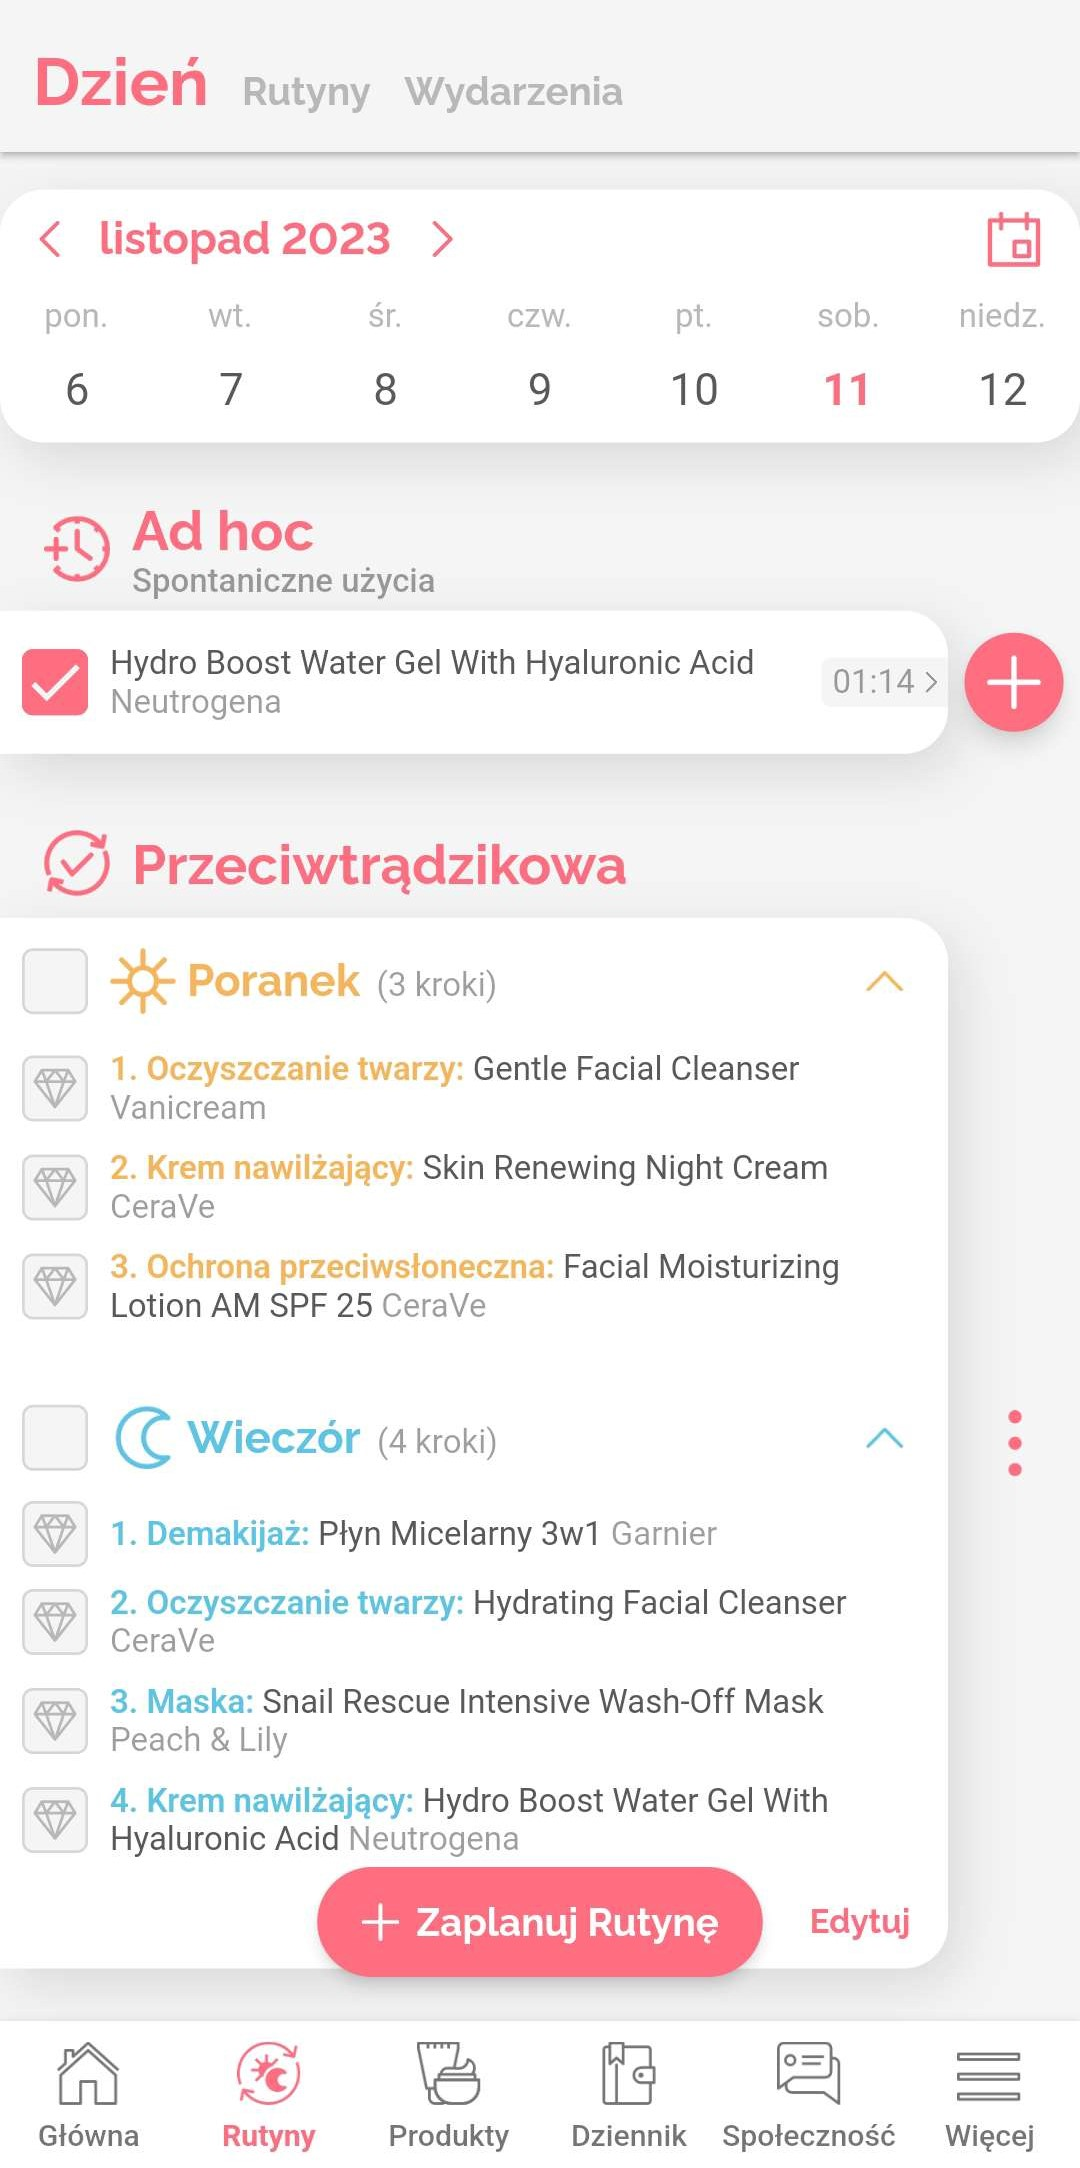
\includegraphics[height=13cm, keepaspectratio]{images/analiza/feelingMySkin}
    \caption{Widok codziennej rutyny w aplikacji FeelingMySkin}
    \label{fig:feelingMySkin}
  \end{minipage}
\end{figure}

ZodiaCal to hybryda wszystkich wymienionych aplikacji.
To minimalistyczne narzędzie służące do wielu celów, ale w podstawowym zakresie.
Próbuje połączyć najlepsze cechy różnych istniejących aplikacji,
oferując minimalistyczny interfejs do zarządzania czasem, zadaniami i nie tylko.
Chociaż nie zawiera wszystkich zaawansowanych funkcji dostępnych w innych aplikacjach,
dąży do dostarczenia użytkownikom wyważonego narzędzia do pracy.

\section{Analiza SWOT}
\phantom{th}
Analiza SWOT to termin powstały od pierwszych liter poszczególnych słów w języku angielskim,
czyli Strengths - siły, Weaknesses - słabości, Opportunities - szanse oraz Threats - zagrożenia.
Jest to metoda analizy rynku, która cieszy się popularnością wśród współczesnych przedsiębiorców.
Takie podejściu do projektu pozwala na lepsze zrozumienie wpływów istniejących już warunków na przyszłość,
szybkie określenie planów strategicznych oraz ułatwia podejmowania decyzji.
Cieszy się popularnością ze względu na prostotę oraz skuteczność działania \cite{businessanalysis}.

\subsubsection*{\textbf{Mocne strony (Strengths):}}
\phantom{Th}
Czynniki aplikacji, które podnoszą jej przewagę konkurencyjną. W tej chwili rynek rozdziela kalendarz osobisty i dzienniczek pielęgnacji na dwie różne aplikację,
co prowadzi do tego, że użytkownik nie tylko musi uzupełniać pola w dwóch różnych miejscach,
uczyć się dwóch różnych interfejsów, ale również przekazywać swoje dane do dwóch różnych serwisów.
Interfejsy wymienionych aplikacji posiadają wiele funkcji do precyzyjnego określania zadań
czy pielęgnacji przez co opanowanie ich zajmuje więcej czasu i wysiłku użytkownika,
niż gdyby posiadały jedynie podstawowe funkcje w tym zakresie.
Aplikacja została stworzona z myślą o wielu platformach dzięki czemu może dotrzeć do szerszej grupy odbiorców.
Opcja, której nie spotkamy w żadnym innym kalendarzu to możliwość sprawdzenia codziennego horoskopu dostosowanego do znaku zodiaku użytkownika.
Dodatkowo, jeśli użytkownik nie wie w jaki sposób określić swój znak zodiaku, aplikacji zrobi to za niego, wystarczy podać dzień i miesiąc urodzenia.

\subsubsection*{\textbf{Słabe strony (Weaknesses):}}
\phantom{Th}
Czynniki aplikacji, które osłabiają jej pozycję. Prostota jest jednocześnie zaletą i wadą. Wadą, ponieważ może nie spełniać oczekiwań zaawansowanych użytkowników,
którym może brakować pewnych funkcji. Brak bazy danych produktów to kolejna słabość projektu.
W aplikacji nie ma możliwości wybrania z bazy danych kosmetyków, których użytkownik używa podczas pielęgnacji jak to mam miejsce w FeelingMySkin.
Opcja ta jest nie dostępna, ponieważ wiązałaby się z podpięciem do przekraczającej wielkościami bazy danych
oraz nieustanne aktualizowanie jej za każdym nowym wprowadzonym produktem na rynek.
Innym negatywnym aspektem jest fakt, iż obecnie rynek przepełniony jest aplikacjami o podobnym charakterze.
W związku z tym konieczne może być przeprowadzenie skutecznej kampanii reklamowej, aby wyróżnić aplikację wśród konkurencji.

\subsubsection*{\textbf{Szanse (Opportunities):}}
\phantom{Th}
Czynniki zewnętrzne, które mają pozytywny wpływ na obecną sytuację na rynku. Ostatnio obserwuje się rosnące zainteresowanie świadomą pielęgnacją skóry,
co przekłada się na wzrost zapotrzebowania na aplikacje ułatwiające planowanie pielęgnacji, czy monitorowanie stanów skóry.


\subsubsection*{\textbf{Zagrożenia (Threats):}}
\phantom{Th}
Czynniki zewnętrzne, które mogą negatywnie wpłynąć na aplikację. Największym wyzwaniem jest zagwarantowanie prywatności i bezpieczeństwa danych.
Konieczne jest zapewnienie wysokiego poziomu ochrony danych użytkowników, zwłaszcza w obszarze związanym z informacjami o pielęgnacji skóry,
które uważane są za dane wrażliwe. Następnym wadliwym punktem są zmiany w regulacjach dotyczących prywatności w różnych państwach.
Zmiany przepisów dotyczących ochrony danych osobowych mogą wymagać dostosowania polityki prywatności aplikacji,
w związku z tym, istotne jest, aby systematycznie monitorować ewentualne zmiany w przepisach.

\section{Analiza przedmiotowa MoSCoW}
\phantom{Th}
Analiza MoSCoW podobnie jak analiza SWOT jest akronimem. Dzieli wymagania na cztery kategorię, uwzględniające wzrastającą złożoność.
Są to kolejno M (Must have) wymagania konieczne, S (Should have) wymagania wskazane, C (Could have) wymagania opcjonalne,
W (Won't have) wymagania wykluczone. Metoda ta pomaga w ustaleniu priorytetów, które w sposób uzasadniony zapewnia kompletny
i dokładny zestaw wymagań, które aplikacja musi spełnić. Takie podejście uświadamia, które funkcje są niezbędne do funkcjonowania systemu
i zapobiega realizacji zadań opcjonalnych przed ukończeniem zadań obowiązkowych. W rezultacie umożliwia bardziej efektywne zarządzanie projektem i zaspokojenie kluczowych potrzeb użytkowników \cite{moscow},\cite{businessanalysis}.

\subsubsection*{\textbf{Must have}}
\phantom{Th}
Zbiór funkcji oznaczony jako Must have to kategorie wymagań, które system jest zobowiązany posiadać.
Podstawowym elementem aplikacji jest połączenie z bazą danych, którą należy w pierwszej kolejności skonfigurować
i podłączyć. Konieczne jest utworzenie modelu danych oraz zapewnienie niezbędnych operacji,
które umożliwią efektywne zarządzanie danymi użytkowników w systemie. Aby korzystać z aplikacji potrzebne jest konto,
co oznacza, że niezbędnym elementem jest ekran logowania i rejestracji.
Ponadto ekrany te muszą posiadać walidację formularzy przed wysłaniem ich na serwer. Zapewni to poprawność
i integralność danych wprowadzanych przez użytkowników oraz pomoże uniknąć potencjalnych błędów
i problemów związanych z danymi przechowywanymi w systemie.

Drugim fundamentem aplikacji jest funkcja kalendarza. Musi ona zapewniać możliwość dodawania, usuwania oraz edytowania wydarzeń, zadań.
Dodatkowo ważnym aspektem jest widok kalendarza na cały rok, miesiąc, tydzień i dzień.
Niezbędną funkcją jest również możliwość rejestrowania swojej pielęgnacji na dany dzień, w zależności od kategorii nawilżanie,
złuszczanie, odbudowa, przerwa. Kolejną kluczową funkcją jest wyświetlanie horoskopu dla znaku zodiaku użytkownika,
co wiąże się ze znalezieniem odpowiedniego API oraz połączenia go z aplikacją.

\subsubsection*{\textbf{Should have}}
\phantom{Th}
W kontekście sekcji Should have skupiamy się na wymaganiach, które są ważne, ale nie są absolutnie niezbędne dla funkcjonowania systemu.
Przydatną funkcją związaną z kalendarzem, z perspektywy użytkownika końcowego jest możliwość automatycznego uzupełnianie pól cyklicznych
takich jak praca/studia oraz otrzymywanie powiadomień. Z kolei rozszerzeniem funkcji pielęgnacji jest opcja związana z dodawaniem
produktów do danej pielęgnacji. Natomiast rozbudowaniem modułu horoskopu jest funkcja przydzielania znaku zodiaku
z podanej daty przez użytkownika. Wiele aplikacji umożliwia logowanie się za pomocą kont z mediów społecznościowych, dlatego warto rozważyć dodanie opcji logowania przy użyciu konta Google, aby sprostać obowiązującym standardom. To umożliwi rozszerzenie funkcjonalności systemu, dostarczając użytkownikom dodatkowych wygodnych i atrakcyjnych opcji.

\subsubsection*{\textbf{Could have}}
\phantom{Th}
Funkcje w grupie Could have to wymagania, które dobrze jest mieć, ale nie są kluczowe.
Dobrym obszarem do rozbudowy jest moduł związany z pielęgnacją.
Można rozszerzyć go o wyświetlaniu wykresów pod koniec miesiąca,
monitorowanie daty ważności używanych produktów oraz dodanie Trackerów samopoczucia, snu i nawyków.
Tracker to narzędzie pozwalające na odnotowanie aktywności w danym stopniu na konkretny dzień.
Na pewno dużym ułatwieniem dal użytkownika byłoby wprowadzenie możliwości zmiany języka oraz onboardingu zaraz po zarejestrowaniu konta.

\subsubsection*{\textbf{Won't have}}
\phantom{Th}
Wymagania w grupie Won't have mają najniższy priorytet. Określają funkcję, które w tej wersji nie zostaną dostarczone,
ale będą zawarte w kolejnej aktualizacji. Klienci często lubią edytować podstawowy interfejs pod siebie,
więc wprowadzenie personalizacji motywów na pewno korzystnie wpłynęłaby na odbiór aplikacji.
Dodatkowo coraz więcej użytkowników decyduje się na smartwatche.
Przyszłościowym krokiem byłoby umożliwienie korzystania z aplikacji również na zegarku.

\chapter{Przegląd technologiczny}
Napisać o systemie kontroli wersji, co to jest Api, o Expo
Korzystać z dokumentacji!!\\

W poniższym rozdziale zostały przedstawione kluczowe technologie potrzebne do wykonania aplikacji.\\
\phantom{Th} 

\section{React Native}\\


\cite{reactnative} React Native to technologia oparta na bibliotece React, która jest używana do tworzenia interfejsów za pomocą języka JavaScript.  Biblioteka ta jest typu open source, co oznacza, że jej kod źródłowy jest udostępniony do użytku publicznego i każdy ma prawo go modyfikować według własnych potrzeb. \\
 
React Native służy do tworzenia wieloplatformowych aplikacji, znanych również jako aplikacje cross-platform, czyli aplikacji zaprojektowanych i napisanych w taki sposób, aby działały na wielu różnych platformach i systemach operacyjnych. Dodatkowo wykorzystuje programowanie natywne zapewniając w ten sposób zestaw komponentów niezależnych od systemu operacyjnego, który następnie jest dynamicznie przekształcany na natywne elementy interfejsu danego systemu. Dzięki temu aplikacja jest w stanie zachować spójność i dostosować się do  konkretnej specyfiki.\\

Wielką zaletą React Native jest jego szybkie odświeżanie, co przyczynia się do oszczędności czasu podczas pisania kodu. Jest to możliwe dzięki wykorzystaniu JavaScript przez React Native.\\


\section{NativeWind}\\

\cite{nativewind} NativeWind wykorzystuje Tailwind CSS jako język skryptowy do tworzenia uniwersalnego systemu styli dla React Native. Z kolei Tailwind CSS to framework do tworzenia interfejsów użytkownika, który opiera się na klasach CSS, ułatwiając tym samym stylizację aplikacji. Framework w tym kontekście to rodzaj struktury lub szkieletu, który zapewnia gotowe rozwiązania, abstrakcje i narzędzia do rozwoju interfejsu. Tailwind CSS dostarcza zestaw predefiniowanych klas CSS, które reprezentują różne style, kolory, marginesy, wypełnienia dzięki czemu interfejs jest konsekwentny i spójny.  \\

Choć React Native nie obsługuje tradycyjnych stylów CSS, narzędzie NativeWind pozwala na przekształcanie klas CSS zapisanych w stylach Tailwind na odpowiednie style i komponenty dostępne w React Native, umożliwiając wykorzystanie tych klas w aplikacjach mobilnych.\\

\section{Expo Go}\\
\cite{expogo} Expo to platforma typu open source dla aplikacji działających natywnie na różnych systemach operacyjnych. Expo umożliwia testowania aplikacji na różnych urządzeniach mobilnych. Aby korzystać z Expo wymagane jest pisanie kodu w JavaScript/TypeScript oraz posiadanie aplikacji na urządeniu mobilnym, które można pobrać z Sklepu Play w przypadku Androida lub z App Store w przypadku iOS'a\\


\section{Google Firebase}\\
Choć React Native nie obsługuje tradycyjnych stylów CSS, narzędzie NativeWind pozwala na przekształcanie klas CSS zapisanych w stylach Tailwind na odpowiednie style i komponenty dostępne w React Native, umożliwiając wykorzystanie tych klas w aplikacjach mobilnych.\\


\section{Postman}\\
Choć React Native nie obsługuje tradycyjnych stylów CSS, narzędzie NativeWind pozwala na przekształcanie klas CSS zapisanych w stylach Tailwind na odpowiednie style i komponenty dostępne w React Native, umożliwiając wykorzystanie tych klas w aplikacjach mobilnych.\\


\section{Visual Studio Code}\\
Choć React Native nie obsługuje tradycyjnych stylów CSS, narzędzie NativeWind pozwala na przekształcanie klas CSS zapisanych w stylach Tailwind na odpowiednie style i komponenty dostępne w React Native, umożliwiając wykorzystanie tych klas w aplikacjach mobilnych.\\


\section{Github}\\
Choć React Native nie obsługuje tradycyjnych stylów CSS, narzędzie NativeWind pozwala na przekształcanie klas CSS zapisanych w stylach Tailwind na odpowiednie style i komponenty dostępne w React Native, umożliwiając wykorzystanie tych klas w aplikacjach mobilnych.\\


\section{Figma}\\
Choć React Native nie obsługuje tradycyjnych stylów CSS, narzędzie NativeWind pozwala na przekształcanie klas CSS zapisanych w stylach Tailwind na odpowiednie style i komponenty dostępne w React Native, umożliwiając wykorzystanie tych klas w aplikacjach mobilnych.\\



\chapter{Wymagania aplikacji}
\section{Analiza przedmiotowa MoSCoW}
\phantom{Th}
Analiza MoSCoW podobnie jak analiza SWOT jest akronimem. Dzieli wymagania na cztery kategorię, uwzględniające wzrastającą złożoność.
Są to kolejno M (Must have) wymagania konieczne, S (Should have) wymagania wskazane, C (Could have) wymagania opcjonalne,
W (Won't have) wymagania wykluczone. Metoda ta pomaga w ustaleniu priorytetów, które w sposób uzasadniony zapewnia kompletny
i dokładny zestaw wymagań, które aplikacja musi spełnić. Takie podejście uświadamia, które funkcje są niezbędne do funkcjonowania systemu
i zapobiega realizacji zadań opcjonalnych przed ukończeniem zadań obowiązkowych. W rezultacie umożliwia bardziej efektywne zarządzanie projektem i zaspokojenie kluczowych potrzeb użytkowników \cite{moscow},\cite{businessanalysis}.

\subsubsection*{\textbf{Must have}}
\phantom{Th}
Zbiór funkcji oznaczony jako Must have to kategorie wymagań, które system jest zobowiązany posiadać.
Podstawowym elementem aplikacji jest połączenie z bazą danych, którą należy w pierwszej kolejności skonfigurować
i podłączyć. Konieczne jest utworzenie modelu danych oraz zapewnienie niezbędnych operacji,
które umożliwią efektywne zarządzanie danymi użytkowników w systemie. Aby korzystać z aplikacji potrzebne jest konto,
co oznacza, że niezbędnym elementem jest ekran logowania i rejestracji.
Ponadto ekrany te muszą posiadać walidację formularzy przed wysłaniem ich na serwer. Zapewni to poprawność
i integralność danych wprowadzanych przez użytkowników oraz pomoże uniknąć potencjalnych błędów
i problemów związanych z danymi przechowywanymi w systemie.

Drugim fundamentem aplikacji jest funkcja kalendarza. Musi ona zapewniać możliwość dodawania, usuwania oraz edytowania wydarzeń, zadań.
Dodatkowo ważnym aspektem jest widok kalendarza na cały rok, miesiąc, tydzień i dzień.
Niezbędną funkcją jest również możliwość rejestrowania swojej pielęgnacji na dany dzień, w zależności od kategorii nawilżanie,
złuszczanie, odbudowa, przerwa. Kolejną kluczową funkcją jest wyświetlanie horoskopu dla znaku zodiaku użytkownika,
co wiąże się ze znalezieniem odpowiedniego API oraz połączenia go z aplikacją.

\subsubsection*{\textbf{Should have}}
\phantom{Th}
W kontekście sekcji Should have skupiamy się na wymaganiach, które są ważne, ale nie są absolutnie niezbędne dla funkcjonowania systemu.
Przydatną funkcją związaną z kalendarzem, z perspektywy użytkownika końcowego jest możliwość automatycznego uzupełnianie pól cyklicznych
takich jak praca/studia oraz otrzymywanie powiadomień. Z kolei rozszerzeniem funkcji pielęgnacji jest opcja związana z dodawaniem
produktów do danej pielęgnacji. Natomiast rozbudowaniem modułu horoskopu jest funkcja przydzielania znaku zodiaku
z podanej daty przez użytkownika. Wiele aplikacji umożliwia logowanie się za pomocą kont z mediów społecznościowych, dlatego warto rozważyć dodanie opcji logowania przy użyciu konta Google, aby sprostać obowiązującym standardom. To umożliwi rozszerzenie funkcjonalności systemu, dostarczając użytkownikom dodatkowych wygodnych i atrakcyjnych opcji.

\subsubsection*{\textbf{Could have}}
\phantom{Th}
Funkcje w grupie Could have to wymagania, które dobrze jest mieć, ale nie są kluczowe.
Dobrym obszarem do rozbudowy jest moduł związany z pielęgnacją.
Można rozszerzyć go o wyświetlaniu wykresów pod koniec miesiąca,
monitorowanie daty ważności używanych produktów oraz dodanie Trackerów samopoczucia, snu i nawyków.
Tracker to narzędzie pozwalające na odnotowanie aktywności w danym stopniu na konkretny dzień.
Na pewno dużym ułatwieniem dal użytkownika byłoby wprowadzenie możliwości zmiany języka oraz onboardingu zaraz po zarejestrowaniu konta.

\subsubsection*{\textbf{Won't have}}
\phantom{Th}
Wymagania w grupie Won't have mają najniższy priorytet. Określają funkcję, które w tej wersji nie zostaną dostarczone,
ale będą zawarte w kolejnej aktualizacji. Klienci często lubią edytować podstawowy interfejs pod siebie,
więc wprowadzenie personalizacji motywów na pewno korzystnie wpłynęłaby na odbiór aplikacji.
Dodatkowo coraz więcej użytkowników decyduje się na smartwatche.
Przyszłościowym krokiem byłoby umożliwienie korzystania z aplikacji również na zegarku.

\section{Wymagania funkcjonalne:}
\phantom{Th}
Podstawowymi funkcjonalnościami jest wszystko to co jest związane z obsługą
kalendarza, czyli dodawanie, usuwanie oraz edycja wydarzeń, zadań, celów czy harmonogramu
na dany dzień, miesiąc. Dodatkowo konieczne jest, aby użytkownik mógł zobaczyć widok
kalendarza na dany miesiąc, tydzień oraz rok. ZodiaCal to nie tylko kalendarz, ale również
dzienniczek pielęgnacji cery. Stąd potrzeba uwzględnienia możliwości wyboru typu pielęgnacji,
dodania, usunięcia, edytowania produktów do danej pielęgnacji oraz funkcja pozwalająca
zarejestrować pielęgnację na dany dzień. Ponadto aplikacja dostarcza codziennie
użytkownikowi horoskop na dany dzień uwzględniając podany wcześniej przez niego znak
zodiaku, lub datę urodzenia.

\section{Wymagania niefunkcjonalne:}
\phantom{Th}
Aby korzystać z aplikacji ZodiaCal, konieczne jest posiadanie telefonu z systemem
Android w wersji 5.0 lub nowszej, lub systemem iOS w wersji 13 lub nowszej. Ponieważ
aplikacja pobiera dane w czasie rzeczywistym i wykorzystuje podstawowy pakiet Firebase,
należy wziąć pod uwagę, że maksymalnie 100 urządzeń może jednocześnie synchronizować się
z bazą danych. Dodatkowo, maksymalna przepustowość danych jest zazwyczaj ograniczona do
360 MB na dzień, co reguluje polityka ograniczeń Firebase \cite{limits}.

\chapter{Projekt interfejsu graficznego}
Dzisiejsze interfejsy graficzne są projektowane zgodnie zasadami User Experience oraz
User Interface. Są to zbiory wytycznych dla projektantów skoncentrowane na doświadczeniach
użytkownika końcowego. User Experience to dziedzina zajmująca się badaniem potrzeb
użytkownika, natomiast User Interface odpowiada za szatę graficzną produktu \cite{uxui}. ZodiaCal zostało stworzone zgodnie z powyższymi zasadami. Poniżej znajdują się Wireframes, czyli modele szkieletowe, zwane również jako architektura widoku aplikacji przedstawiające projekt graficzny poszczególnych ekranów wykonem w aplikacji internetowej Figma. Są to High-Fidelity Wireframes, co oznacza, że stanowią dopracowane rozwiązanie z szczegółowymi detalami \cite{uxui}.


\begin{figure}[h]
	\begin{minipage}{0.3\textwidth}
		\centering
		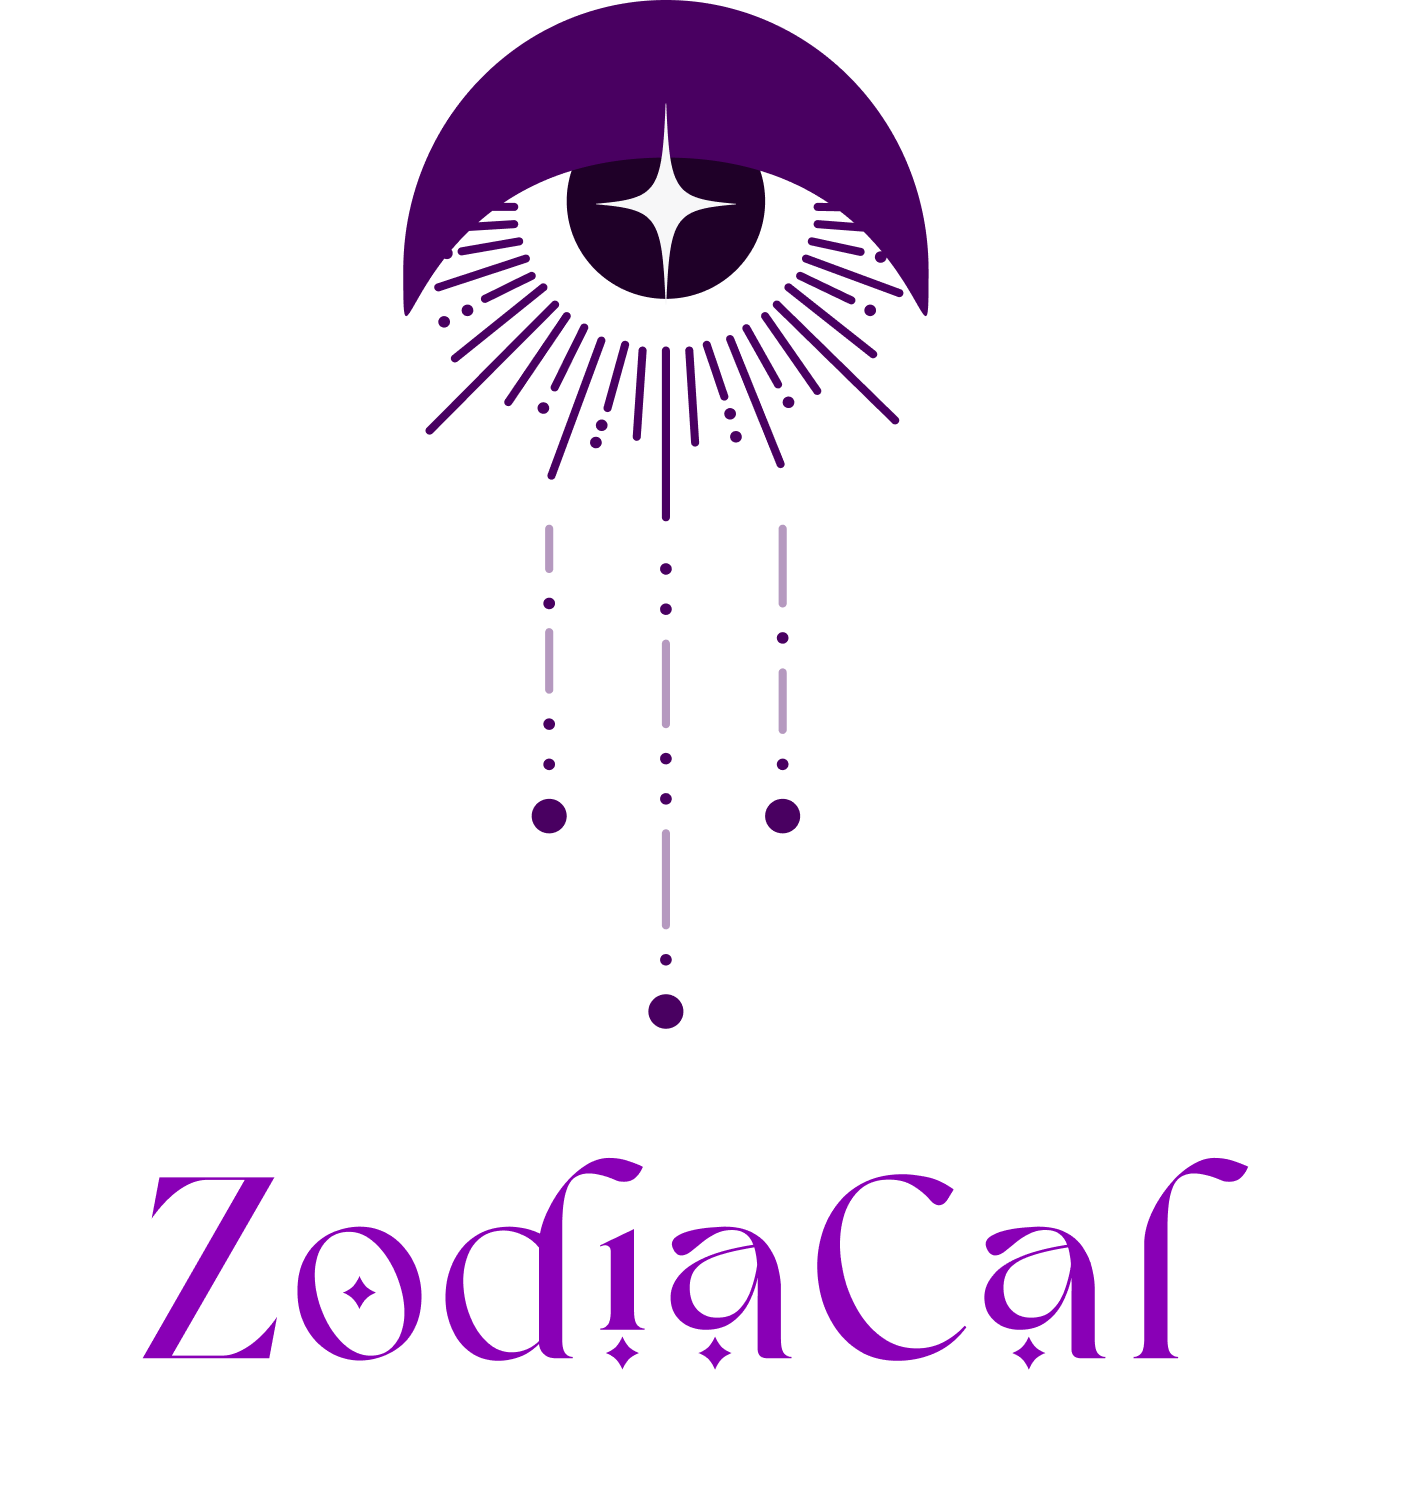
\includegraphics[height=4cm, keepaspectratio]{images/logo/logo_text}
		\caption{Logo wraz z typografią}
		\label{fig:logo_text}
	\end{minipage}
	\hfill
	\begin{minipage}{0.3\textwidth}
		\centering
		
\includegraphics[height=4cm, keepaspectratio]{images/logo/logo}
		\caption{Logo bez typografii}
		\label{fig:logo}
	\end{minipage}
	\hfill
	\begin{minipage}{0.3\textwidth}
		\centering
		
\includegraphics[height=4cm, keepaspectratio]{images/logo/favicon}
		\caption{Ikona aplikacji favicon}
		\label{fig:favicon}
	\end{minipage}
\end{figure}

Rysunek \ref{fig:logo_text} przedstawia logo aplikacji ZodiaCal. Zostało one zaprojektowane z wykorzystaniem narzędzia Figma, który umożliwia tworzenie obrazów wektorowych, to znaczy obrazów opisanych za pomocą kształtów, linii i krawędzi w odróżnieniu do grafiki rastrowej opartej na pikselach. Dzięki wykorzystaniu wektorów grafiki nie tracą swojej ostrości
podczas powiększani, czy zmieniania obiektu. Stworzone logo miała nawiązywać do astrologicznych motywów tak, aby przywodziło na myśl horoskopy oraz wróżbiarstwo. Font wykorzystany do nazwy aplikacji został staranie wybrany, aby oddać charakter aplikacji. Jest to
font szeryfowy posiadający małe dekoracyjne elementy. Wykorzystanie takie rodzaju typografii ma na celu wywołanie wrażenia, że aplikacja prezentuje się w sposób klasyczny i elegancki.


\begin{figure}[t]
	\begin{minipage}{0.4\textwidth}
		\centering
		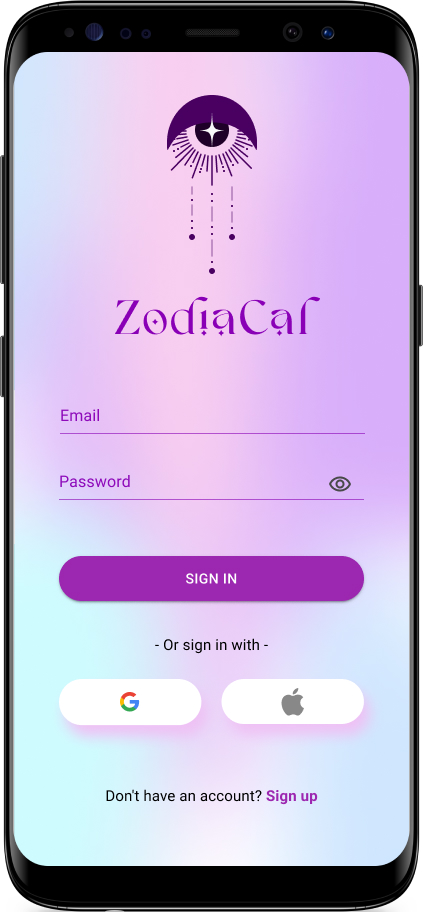
\includegraphics[height=10cm, keepaspectratio]{images/interfejs_figma/Sign_in}
		\caption{Ekran logowania}
		\label{fig:Sign-in}
	\end{minipage}
	\hfill
	\begin{minipage}{0.4\textwidth}
		\centering
		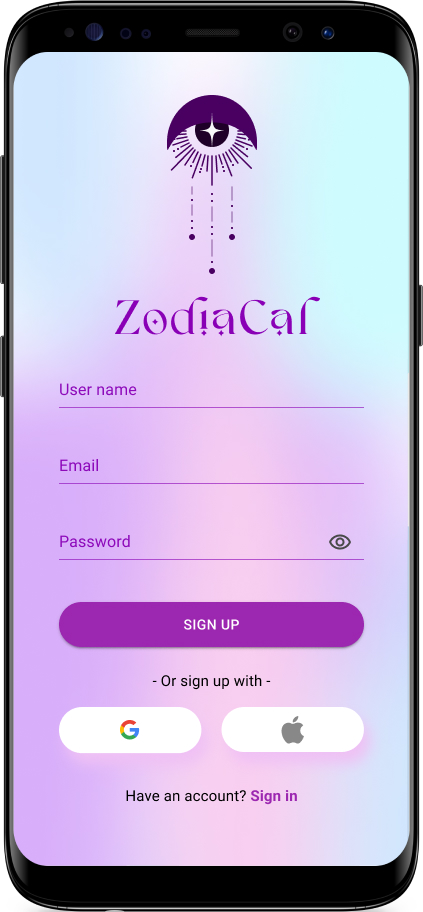
\includegraphics[height=10cm,           keepaspectratio]{images/interfejs_figma/Sign_up}
		\caption{Ekran rejestracji}
		\label{fig:Sign-up}
	\end{minipage}
\end{figure}

\section{Projekt ekranu logowania}
Ekran logowania (Rys. \ref{fig:Sign-in}) przedstawia minimalistyczny formularz logowania do aplikacji, który zawiera dwa pola umożliwiające wprowadzeniu tekstu typu TextInput. TextInputy są interaktywne, to znaczy, że reagują na dane wpisane przez użytkownika. Takie rozwiązanie pozwala na komunikację klienta z aplikacją w celu uniknięcia błędów podczas wpisywania tekstu oraz frustracji użytkownika, który bez komunikatu nie wiedziałby co się dzieje na ekranie. Pole z hasłem ma ikonę oczka, dzięki której można podejrzeć wpisane hasło. Dodatkowo użytkownik ma możliwość zalogowania się do aplikacji poprzez serwisy społecznościowe takie jak konto Google, czy konto Apple. Jeśli klient nie ma jeszcze zarejestrowanego konta może przejść do ekranu rejestracji klikając w przycisk „Sign up”.

\section{Projekt ekranu rejestracji}
Rejestracja użytkownika (Rys. \ref{fig:Sign-up}) odbywa się poprzez uzupełnienie trzech pól w formularzu. Podobnie jak w przypadku ekranu logowania pole „Password” posiada ikonę oczka oraz możliwe jest utworzenie konta z wykorzystaniem innych kont społecznościowych. Po poprawnym wprowadzeniu danych i kliknięciu przycisku „Sign up”, użytkownik zostaje
przeniesiony do ekranu głównego aplikacji.

\begin{figure}[t]
	\begin{center}
		\begin{minipage}{0.4\textwidth}
			\centering
			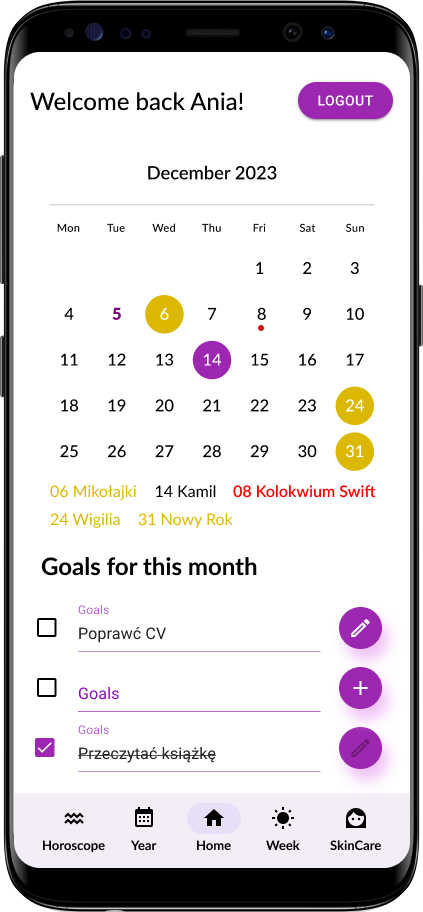
\includegraphics[height=10cm, keepaspectratio]{images/interfejs_figma/Home}
			\caption{Ekran główny}
			\label{fig:Home}
		\end{minipage}
	\end{center}
\end{figure}

\section{Projekt ekranu głównego}
Po udanym zalogowaniu się do aplikacji, użytkownik jest powitany spersonalizowanym komunikatem, który zawiera jego imię (Rys. \ref{fig:Home}). Dodatkowo w tej samej płaszczyźnie znajduję się przycisk do wylogowania. Poniżej znajduję się kalendarz miesięczny z zaznaczonymi świętami, wydarzeniami oraz urodzinami użytkownika. Wygubiony numer w kolorze fioletowym reprezentuje obecny dzień, numer w żółtym kole oznacza święto, numer w fioletowym kole informuje o urodzinach bliskich, mała czerwona kropeczka pod numerem wskazuje na nadchodzące wydarzenie. Pod kalendarzem zostały umieszczone wszystkie informację o zaznaczonych polach w kalendarzu. Dodatkowo poniżej znajduje się sekcja „Goals for this month” w której użytkownik może wprowadzić trzy cele, które chciałby osiągnąć w danym miesiącu. Każde pole posiada checkbox, który informuje, czy klient ukończył cel, jeśli tak checkbox zostaje wypełniony kolorem fioletowym, a tekst w polu zostaje przekreślony, opcja edytowania tekstu zostaje wyłączona. Po prawej stronie znajdują się okrągłe przyciski. Jeśli pole jest puste, przyciski reprezentuje plusik, jeśli w polu już cos się znajduje ikona zmienia się na ołówek, co oznacza, że pole można edytować. W całej aplikacji została wprowadzona nawigacja dolna. Zawiera ona ikony i nazwy odzwierciedlające dostępne ekrany. Zawsze aktualny ekran jest wyróżniony w pasku nawigacyjnym.

\begin{figure}[t]
	\begin{minipage}{0.4\textwidth}
		\centering
		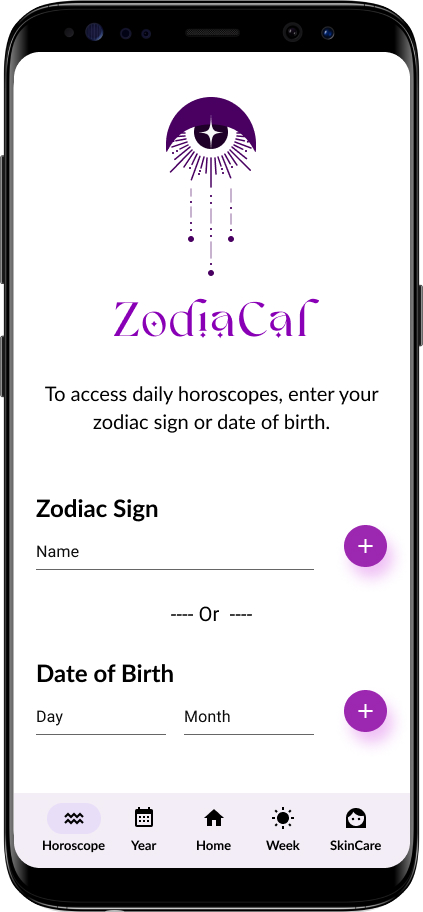
\includegraphics[height=10cm, keepaspectratio]{images/interfejs_figma/Horoscope-onboarding}
		\caption{Onboarding horoskopu}
		\label{fig:Onboarding}
	\end{minipage}
	\hfill
	\begin{minipage}{0.4\textwidth}
		\centering
		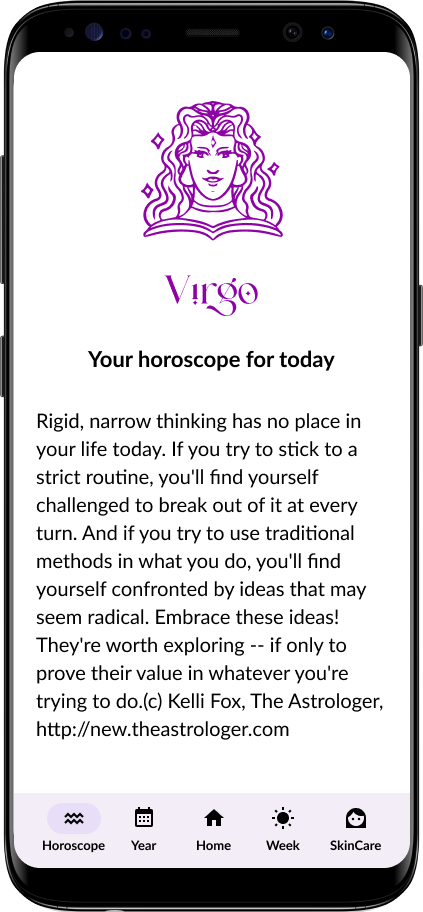
\includegraphics[height=10cm,           keepaspectratio]{images/interfejs_figma/Horoscope}
		\caption{Ekran dziennego horoskopu}
		\label{fig:Horoscope}
	\end{minipage}
\end{figure}

\section{Projekt ekranu horoskopu}
Pierwszą zakładką w nawigacji jest ekran horoskopu, który może wyglądać na dwa sposoby w zależności od tego, czy użytkownik wprowadził swój znak zodiaku do systemu.

Pierwszy scenariusz został ukazany na rysunku \ref{fig:Onboarding}. Jeśli klient uruchamia tę zakładkę po raz pierwszy, jego oczom ukaże się logo aplikacji oraz dwa małe formularze. Użytkownik, jeśli zna swój znak zodiaku może go wprowadzić w pierwszym formularzu. Jeśli jednak dopiero rozpoczyna swoją przygodę z horoskopami, aplikacja pomoże mu określić swój znak zodiaku. Wystarczy podać dzień i miesiąc urodzenia, a program sam przydzieli znak zodiaku i wyświetli go na ekranie wraz z horoskopem.

Rysunek \ref{fig:Horoscope} przedstawia sytuację, gdzie w systemie już znajduję się informacja o znaku zodiaku użytkownika. Logo aplikacji zostaje zamienione na ilustrację przetrawiającą wersję graficzną znaku zodiaku. Ilustracje wszystkich znaków zostały pobrane ze strony Freepik.com, który posiada darmową licencję do korzystania z zasobów znajdujących się na stronie w zakresie niekomercyjnym. Każdego dnia na tym ekranie pojawia się inna wróżba zodiaku.

\begin{figure}[t]
	\begin{minipage}{0.4\textwidth}
		\centering
		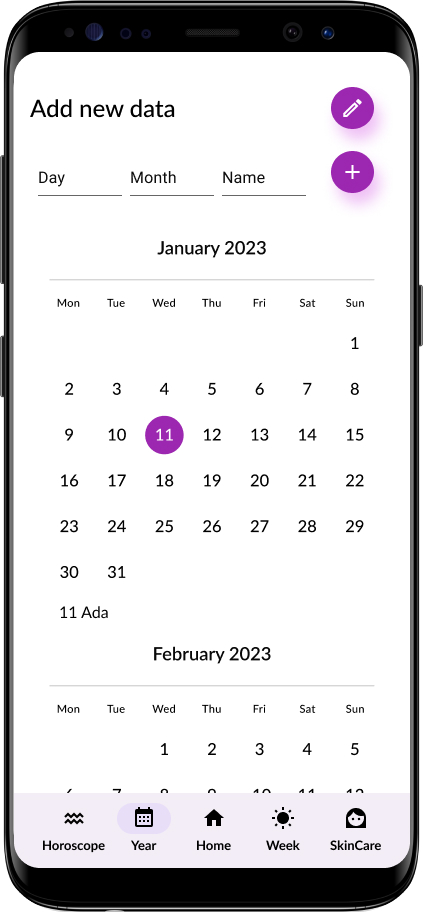
\includegraphics[height=10cm, keepaspectratio]{images/interfejs_figma/Year}
		\caption{Widok kalendarza rocznego}
		\label{fig:Year}
	\end{minipage}
	\hfill
	\begin{minipage}{0.4\textwidth}
		\centering
		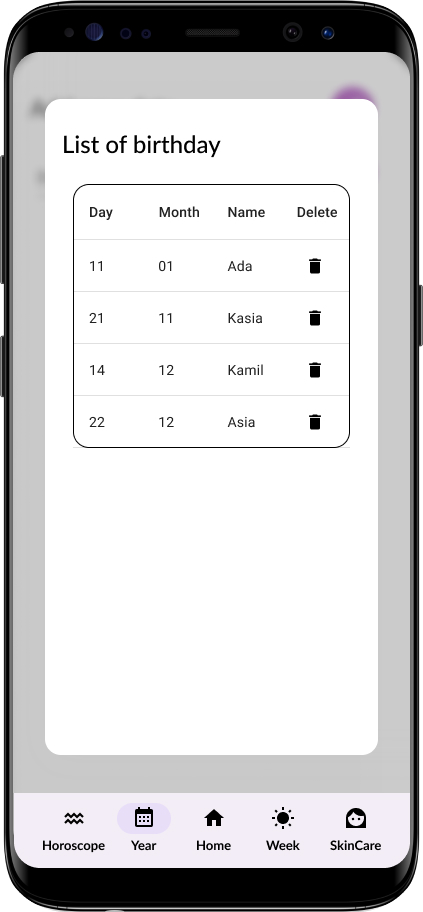
\includegraphics[height=10cm,           keepaspectratio]{images/interfejs_figma/Birthday-Edit}
		\caption{Ekran listy dat urodzin}
		\label{fig:Birthday}
	\end{minipage}
\end{figure}

\section{Projekt widoku kalendarza rocznego}
Kolejna zakładka o nazwie „Year” przenosi użytkownika do widoku kalendarza rocznego \ref{fig:Year}). W tym ekranie wyświetlane są kalendarze miesięcy jedynie danego roku. Dzięki takiemu rozwiązaniu klient nie musi się przejmować zbędnym skorolowaniem, które może omyłkowo zaprowadzić go do zupełnie innego roku. W tym widoku kalendarza zaznaczone są jedynie święta oraz urodziny. Poniżej każdego kalendarza na dany miesiąc znajduję się informacja o zaznaczonych polach. Na górze ekranu został umieszczony formularz do dodawania urodziny do listy użytkownika. Zawiera on trzy pola: day, month oraz name. Po prawej stronie znajduje się przycisk dodawania urodzin do listy. Jeśli użytkownik się pomyli lub
po prosu będzie chciał edytować listę z datami, musi kliknąć w okrągły przycisk z ikoną ołówka. Otworzy się wtedy tak zwany portal (Rys. \ref{fig:Birthday}) przedstawiający tabelę z czterema kolumnami: day, month, name i delete. To właśnie tam użytkownik może usunąć złe rekordy. Tabela sortuję się w taki sposób, aby na początku zawsze były pola z poprawną kolejnością miesięcy, a następnie w sposób rosnący reprezentuje kolejność dni w miesiącu.

\begin{figure}[t]
	\begin{minipage}{0.4\textwidth}
		\centering
		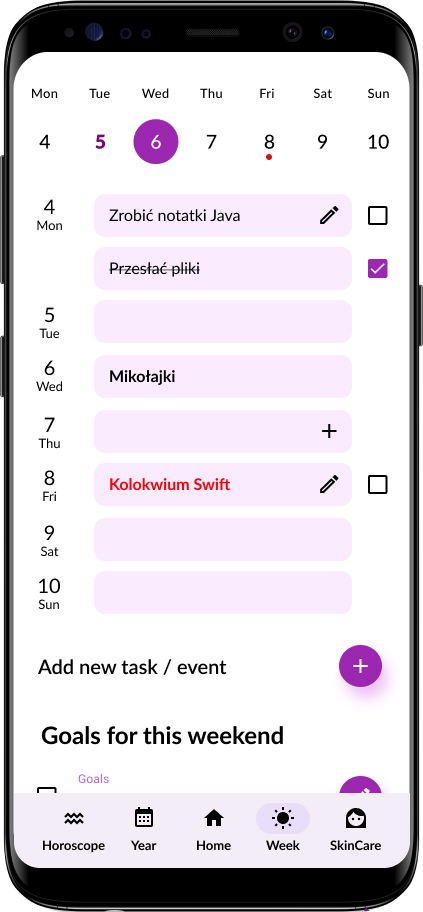
\includegraphics[height=10cm, keepaspectratio]{images/interfejs_figma/Week}
		\caption{Widok kalendarza tygodniowego}
		\label{fig:Week}
	\end{minipage}
	\hfill
	\begin{minipage}{0.4\textwidth}
		\centering
		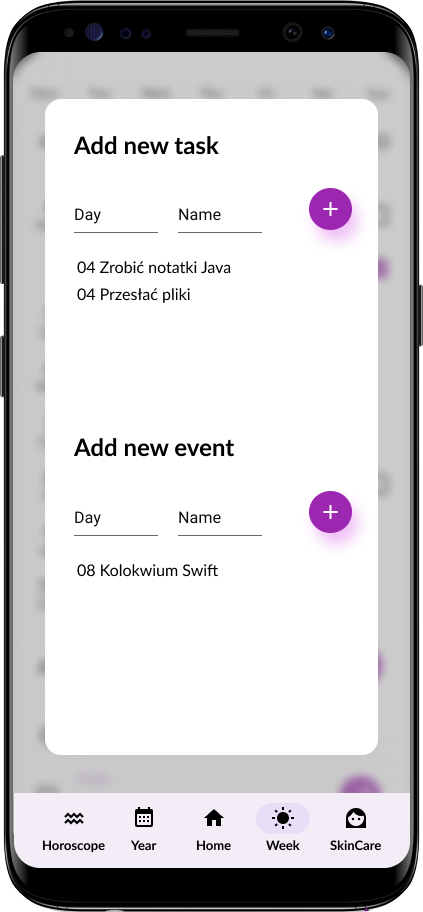
\includegraphics[height=10cm,           keepaspectratio]{images/interfejs_figma/Task_Event}
		\caption{Ekran dodawania zadań i wydarzeń do kalendarza}
		\label{fig:Task_Event}
	\end{minipage}
\end{figure}

\section{Projekt widoku kalendarza tygodniowego}
Rysunek \ref{fig:Week} reprezentuje ekran zakładki „Week”. W tym widoku  użytkownik może podglądać swoje zadania i wydarzenia na konkretny tydzień. Na samej górze znajduje się kalendarz z pogrubionym obecnym dniem, zaznaczonym świętem i wydarzeniem. Poniżej dla każdego dnia zostają wyświetlone zdania i wydarzenia, które użytkownik wprowadził na dany dzień. Klient może edytować pola zadań i wydarzeń poprzez kliknięcie ikony ołówka. Inputy mają takie samo zachowanie jak w przypadku komponentu Goals w ekranie głównym. Na samym dole znajduje się miejsce na wpisanie przez użytkownika celów na ten tydzień.

Aby dodać zadanie lub wydarzenie należy kliknąć okrągły przycisk z plusem. Po tej akcji pojawi się portal z formularzem do tworzenia zadań i wydarzeń (Rys. \ref{fig:Task_Event}). Jest to bardzo minimalistyczny interfejs zawierający dwa TextInput day i name oraz przycisk dodawania. Aby zachować spójność projektu poniżej każdego z formularzy znajduje się tabela z trzema kolumnami: day, name, delete. Z tego miejsca użytkowni może zarządzać swoimi zadaniami oraz wydarzeniami na dany tydzień. Tabela sortuje rekordy w sposób rosnący.

\begin{figure}[t]
	\begin{center}
		\begin{minipage}{0.4\textwidth}
			\centering
			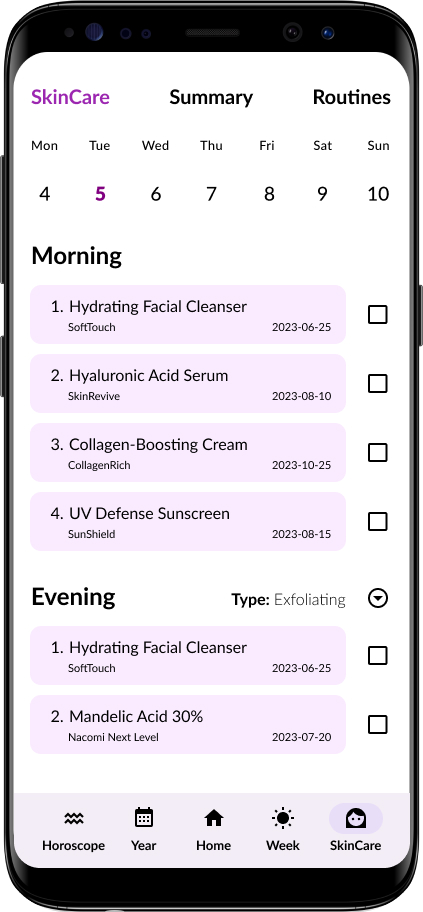
\includegraphics[height=10cm, keepaspectratio]{images/interfejs_figma/SkinCare}
			\caption{Ekran pielęgnacji na dany dzień}
			\label{fig:SkinCare}
		\end{minipage}
	\end{center}
\end{figure}

\section{Projekt ekranu pielęgnacji}
Ostatnią zakładką w pasku nawigacyjnym jest SkinCare (Rys. \ref{fig:SkinCare}). Podobnie jak w ekranie widoku kalendarza tygodniowego na górze znajduje się kalendarz tygodniowy, z tym że na nim nie ma już zaznaczonych żadnych świąt, wydarzeń czy zadań. Dodatkowo klikając w poszczególne dni na kalendarzu poniżej wyświetla się pielęgnacja dedykowana na konkretny dzień, w ekranie widoku kalendarza tygodniowego, wszystkie zadania, wydarzenia, święta są wyświetlane razem. Pielęgnacja jest podzielona na dwie sekcje: pielęgnację poranną i pielęgnację wieczorną. Pielęgnacja na dzień zawsze zawiera te same produkty, chyba że użytkownik sam je zmieni, natomiast pielęgnacja na wieczór jest wybierana z wysuwanego menu z którego można wybrać jedną z czterech typów pielęgnacji: nawilżająca, złuszczająca, regeneracyjna lub przerwa. W zależności od tego jaką pielęgnacje użytkownik wybierze taka lista produktów zostanie wyświetlona w sekcji pielęgnacji wieczornej. Dodatkową funkcją jest możliwość kliknięcia przez użytkownika checkboxa, gdy wykorzystał produkt z wymienionej listy. Na samej górze znajduję się osobna mini nawigacja dla sekcji SkinCare. Aktualny widok jest zaznaczony kolorem fioletowym w nawigacji.

\begin{figure}[t]
	\begin{minipage}{0.4\textwidth}
		\centering
		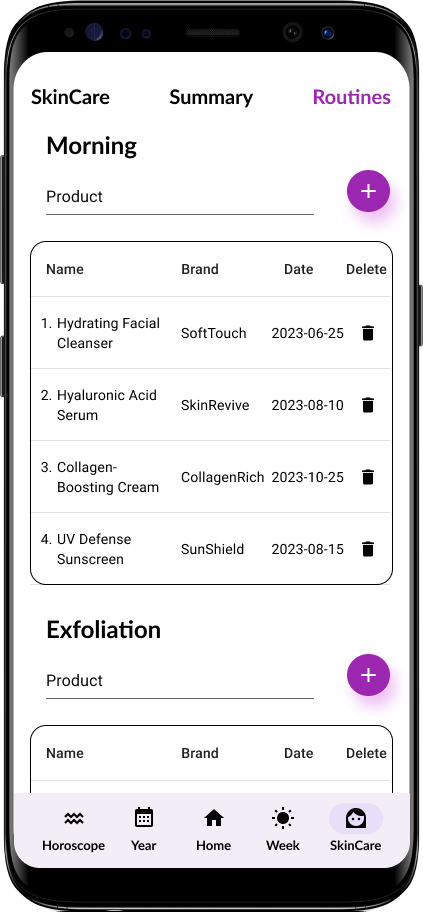
\includegraphics[height=10cm, keepaspectratio]{images/interfejs_figma/SkinCare-Routines}
		\caption{Ekran tworzenia rutyny pielęgnacyjnej}
		\label{fig:Routines}
	\end{minipage}
	\hfill
	\begin{minipage}{0.4\textwidth}
		\centering
		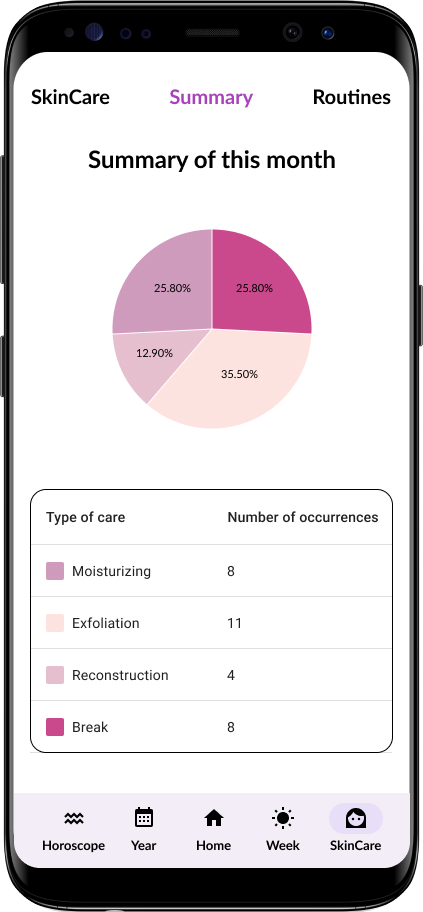
\includegraphics[height=10cm,           keepaspectratio]{images/interfejs_figma/SkinCare-Summary}
		\caption{Ekran podsumowania miesiąca pielęgnacji}
		\label{fig:Summary}
	\end{minipage}
\end{figure}

Początkowo sekcja pielęgnacji porannej i wieczornej jest pusta, aby dodać kosmetyki należy kliknąć Rutines w górnej nawigacji. Po wykonaniu tego kroku użytkownikowi ukażą się formularze z nagłówkiem oraz polem do wpisania (Rys. \ref{fig:Routines}). Podczas wpisywania nazwy klient będzie mógł wybrać z bazy danych konkretne produkty. Po dodaniu produktu poniżej zostanie zaktualizowana tabela z listą produktów do danej pielęgnacji. W tabeli znajdują się cztery kolumny: name, brand, date oraz delete. Dla każdej sekcji jest osobny formularz oraz tabela. Ostatnim ekranem jest widok podsumowania pielęgnacji na dany miesiąc (Rys. \ref{fig:Summary}).

W tym miejscu są wyświetlane informacja w jakim stopniu pielęgnacja w tym miesiącu była nawilżająca, złuszczająca, regeneracyjna lub wystąpiła przerwa. Na środku znajduję się graf kołowy z wypisanymi procentami, a poniżej tabela z dwiema kolumnami: „Type of care” stanowiąca również legendę do wykresu oraz  „Number of occurrences”, która wyświetla ile razy dana pielęgnacja wystąpiła w miesiącu.



\chapter{Model danych}
\addcontentsline{toc}{chapter}{Model danych}
Diagramy UML zwane również Unified Modeling Language umożliwiają graficzne przedstawienie logiki relacji, czy procesu \cite{diagram}. Są to standardy graficzne używane w inżynierii oprogramowania do modelowania struktury i zachowania systemów informatycznych. Umożliwiają one lepsze zrozumienie architektury systemu oraz pomagają w procesie projektowania i dokumentowania. Poniżej zostały przedstawione diagramy kolekcji występujących w bazie danych Firebase wykorzystywanych w aplikacji ZodiaCal.

\section*{Diagram bazy danych}
\addcontentsline{toc}{section}{Diagram bazy danych}

\begin{figure}[h]
	\centering
	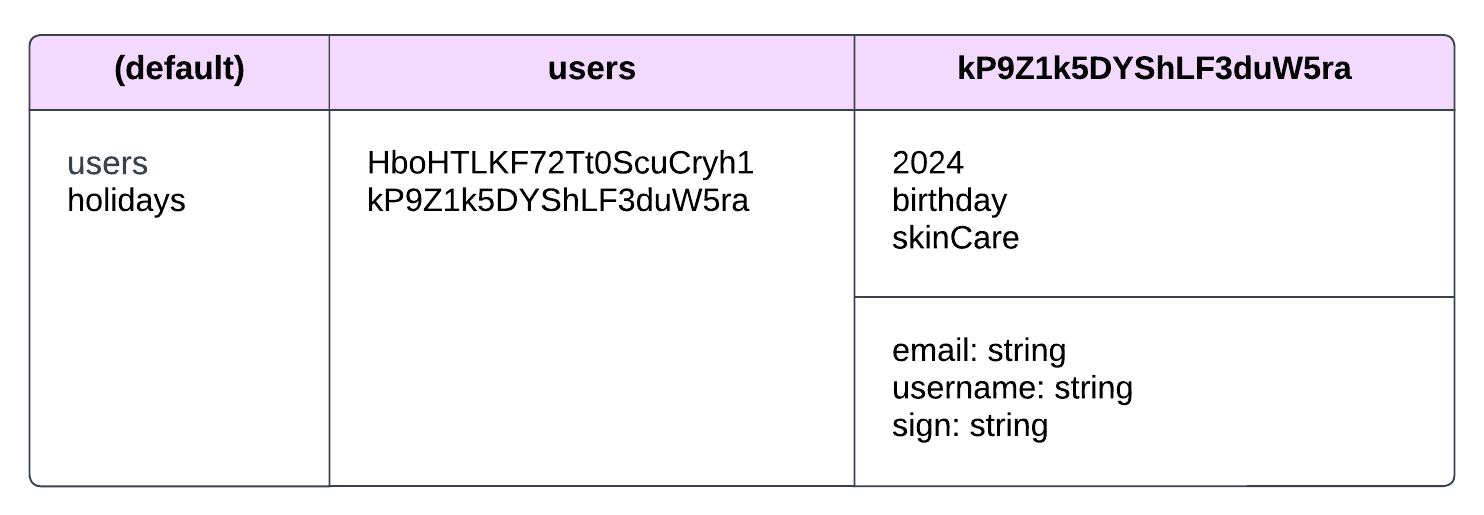
\includegraphics[width=1\linewidth]{images/model_danych/user}
	\caption{Diagram kolekcji user}
	\label{fig:user}
\end{figure}

Diagram kolekcji user (Tab. \ref{fig:user}) zawiera informację o zalogowanym użytkowniku. Każdy user posiada swój własny unikalny User UID. Podstawowe dane użytkownika to obowiązkowe pola email i user name oraz opcjonalne pole sign. Podczas korzystania z aplikacji w bazie danych tworzą się kolekcje takie jak obecny rok, w którym przechowywane są wszystkie informacje potrzebne do zarządzania kalendarzem, kolekcja birthday, w której użytkownik przechowuje daty urodzin swoich bliskich oraz kolekcję skinCare przechowujące treści dotyczące pielęgnacji cery.

\newpage

\begin{figure}[h]
	\centering
	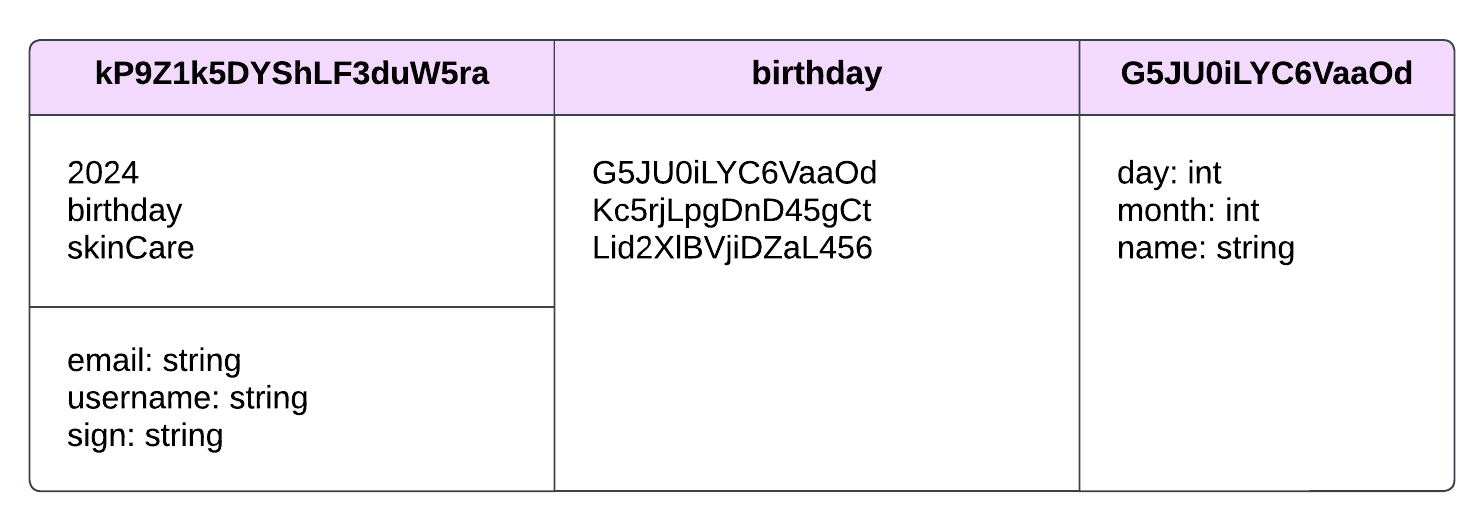
\includegraphics[width=1\linewidth]{images/model_danych/birthday}
	\caption{Diagram kolekcji birthday}
	\label{fig:birthday}
\end{figure}

Kolekcja birthday (Tab. \ref{fig:birthday}) przedstawia listę dat urodzin różnych osób. Posiada dwa pola typu int tzn. day oraz month i jedno pole typu string name, które wskazuje na imię jubilata.

\begin{figure}[h]
	\centering
	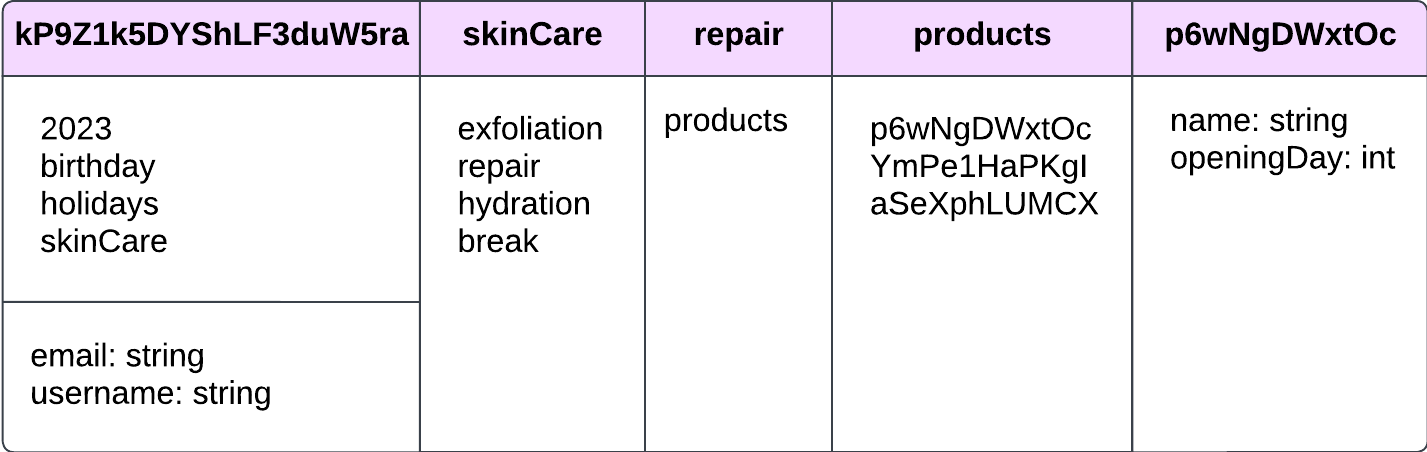
\includegraphics[width=1\linewidth]{images/model_danych/skinCare}
	\caption{Diagram kolekcji skinCare}
	\label{fig:skinCare}
\end{figure}

W tabeli o nazwie "skinCare" (Tab. \ref{fig:skinCare}), znajduje się zbiór informacji dotyczących pielęgnacji cery. W ZodiaCal zostały wyróżnione 4 rodzaje pielęgnacji: złuszczanie, odbudowa, nawilżanie oraz przerwa. Każda kolekcja danego typu pielęgnacji posiada swoje własne produkty. Produkty natomiast zawierają informację o nazwie produktu, nazwie marki oraz terminie ważności kosmetyku. Użytkownik wybiera produkty do pielęgnacji z zewnętrznego API, a następnie są one przekazywane do Firebase.

\begin{figure}[h]
	\centering
	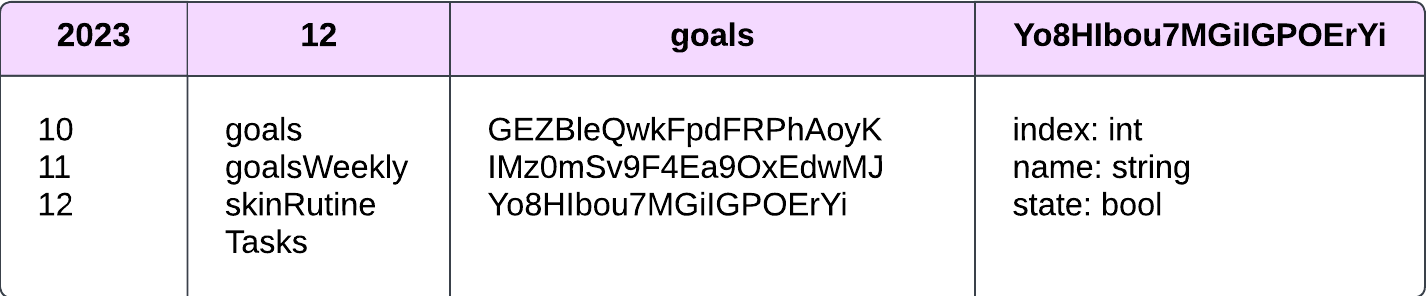
\includegraphics[width=1\linewidth]{images/model_danych/goals}
	\caption{Diagram kolekcji goals}
	\label{fig:goals}
\end{figure}

Kolekcja goals (Tab. \ref{fig:goals}) jest zagnieżdżona kolejno w kolekcji reprezentujący bieżący rok następnie bieżący miesiąc. W kolekcji odzwierciedlającej bieżący miesiąc znajdują się kolekcje dotyczące celi na dany miesiąc oraz tydzień, rutyny pielęgnacyjnej oraz zadań. Każdy cel ma swój unikalny ID, pole typu int przechowujące numer indexu, pole typu string name przedstawiające cel oraz pole typu bool state, które wskazuje czy cel został osiągnięty, czy nie.

\begin{figure}[h]
	\centering
	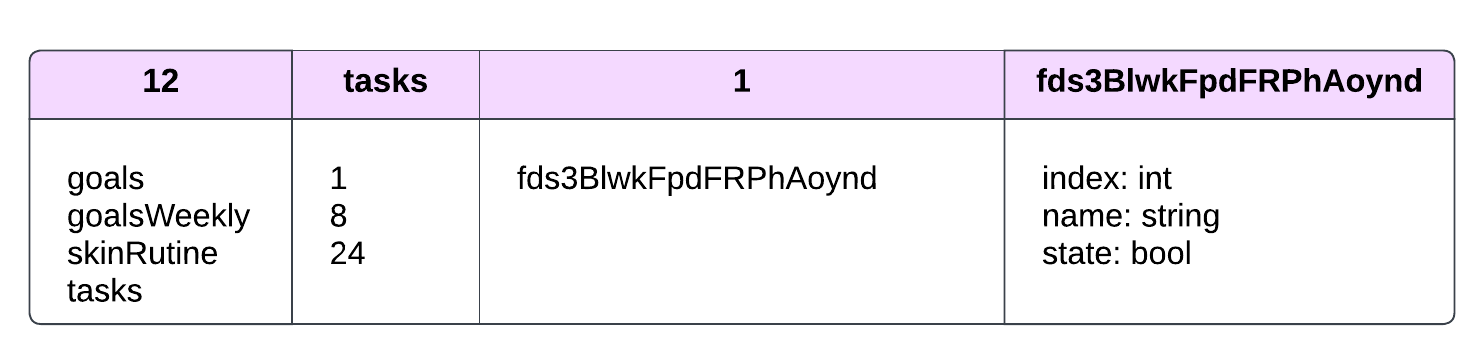
\includegraphics[width=1\linewidth]{images/model_danych/tasks}
	\caption{Diagram kolekcji tasks}
	\label{fig:tasks}
\end{figure}

Podobnie jak w przypadku kolekcji goals, tabela zatytułowana tasks (Tab. \ref{fig:tasks}) również jest zagnieżdżona w bieżącym roku oraz miesiącu. W tej kolekcji są tworzone kolejne kolekcje ilustrujące dni w danym miesiącu. Wszystkie zadania są przypisane do swoich unikalnych identyfikatorów, posiadają pola typu int, w których przechowywane są numery indeksów, pola typu string oznaczone jako "name" zawierające opis zadania, a także pola typu bool oznaczone jako "state", wskazujące na stan zadania.

\section*{Diagram UML komponentów}
\addcontentsline{toc}{section}{Diagram UML komponentów}

\begin{figure}[h]
	\centering
	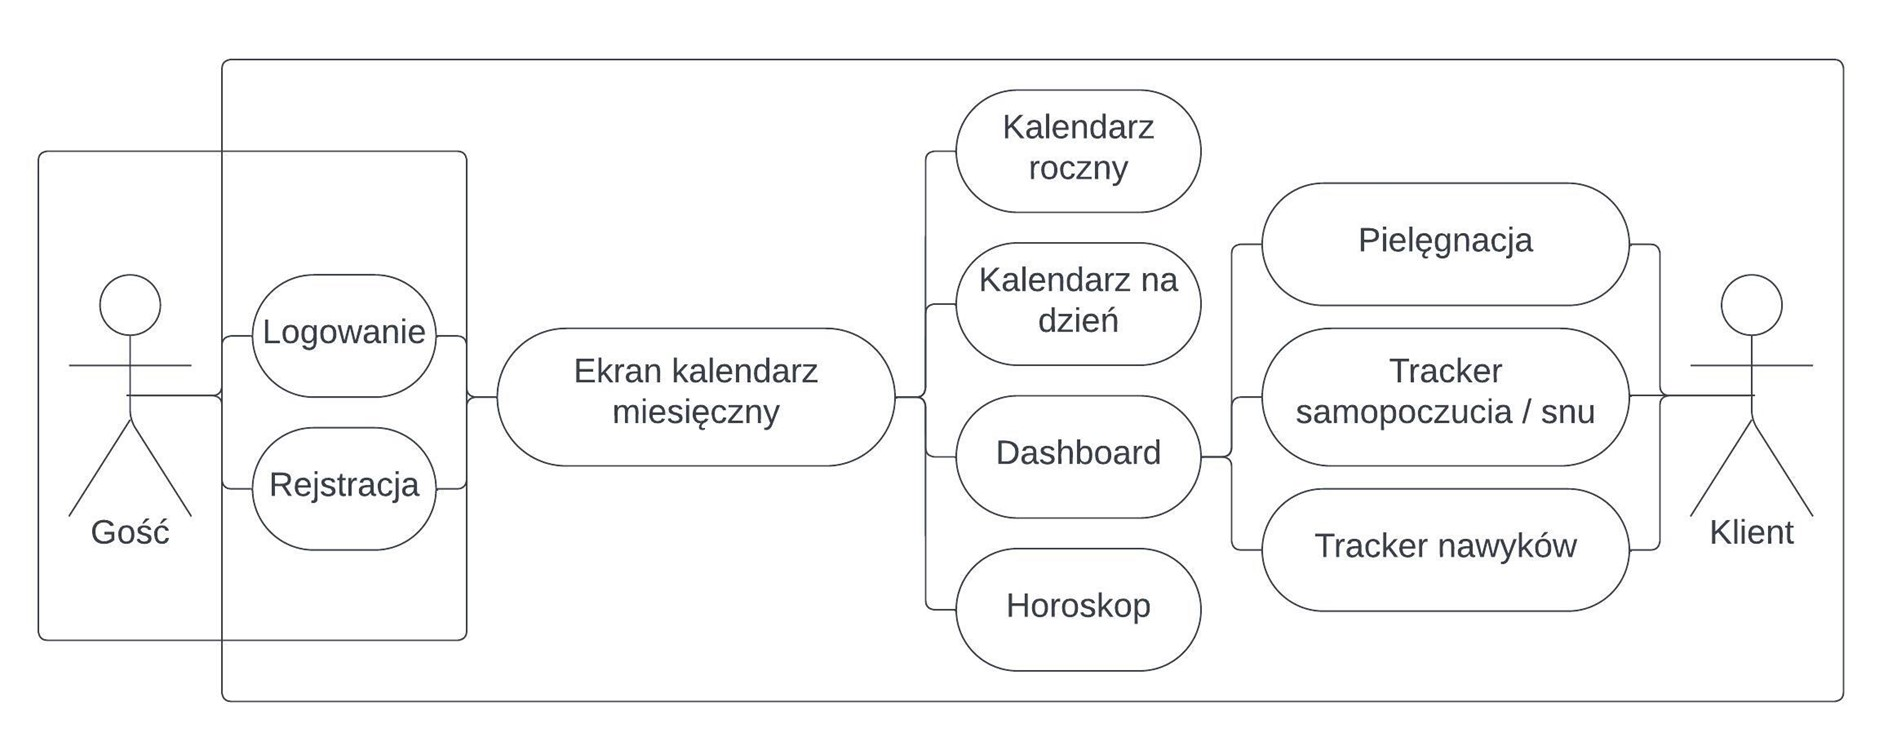
\includegraphics[width=1\linewidth]{images/model_danych/uml}
	\caption{Diagram UML komponentów}
	\label{fig:uml}
\end{figure}

NAPISAĆ CZYM SĄ KOMPONENTY!

\section*{Diagram przypadków użycia}
\addcontentsline{toc}{section}{Diagram przypadków użycia}

SKOMPRESOWAĆ ODSTĘPY + NUMERKI ZAMIAST LITER W PODLIŚCIE! + WCIĘCIE PRZYPADEK UŻYCIA

\textbf{Przypadek użycia:} Rejestracja użytkownika

\textbf{Aktor:} Gość

\textbf{Opis:} Przypadek użycia "Rejestracja użytkownika" umożliwia nowym użytkownikom stworzenie konta w systemie. Rejestracja wymaga podania informacji, takich jak nazwę, adres e-mail, dzień urodzenia oraz hasło. Umożliwia to dostęp do pełnych funkcji systemu, takich jak logowanie, przeglądanie zawartości i zarządzanie swoim profilem.

\textbf{Warunki wstępne:} Gość odwiedza stronę rejestracji. Gość nie posiada konta w systemie.

\textbf{Przebieg:}

\begin{enumerate}
	\item Gość wchodzi na ekran rejestracji.
	\item System wyświetla formularz rejestracyjny.
	\item Gość wprowadza swoje dane, takie jak nazwę, adres e-mail, hasło oraz dzień urodzenia
	\item System sprawdza poprawność wprowadzonych danych.
	\begin{enumerate}
		\item Wprowadzone dane są poprawne.
		\begin{enumerate}
			\item Gość jest automatycznie zalogowany na nowo utworzone konto.
		\end{enumerate}
		\item Wprowadzone dane są niepoprawne.
		\begin{enumerate}
			\item Zostaje wyświetlony komunikat, że podane dane są niepoprawne. Użytkownik nie zostaje dodany do bazy danych.
		\end{enumerate}
	\end{enumerate}
\end{enumerate}


\textbf{Przypadek użycia:} Logowanie użytkownika

\textbf{Aktor:} Gość

\textbf{Opis:} Przypadek użycia "Logowanie użytkownika" umożliwia użytkownikom dostęp do
pełnych funkcji systemu. Logowanie wymaga podania informacji, takich jak adres e-mail
i hasło.

\textbf{Warunki wstępne:} Gość uruchamia aplikację. Użytkownik niezalogowany w serwisie.

\textbf{Przebieg:}


\textbf{Przypadek użycia:} Sprawdzenie horoskopu

\textbf{Aktor:} Klient

\textbf{Opis:} Przypadek użycia "Sprawdzenie horoskopu" umożliwia użytkownikom dostęp do
codziennych horoskopów dedykowany dla ich znaku zodiaku.

\textbf{Warunki wstępne:} Klient ma przydzielony znak zodiaku z bazy danych.

\textbf{Przebieg:}
\begin{enumerate}
	\item Klient przesuwa ekran w prawą stronę.
	\item Zostaje wyświetlona nazwa znaku zodiaku, ilustracja oraz horoskop na dany dzień.
\end{enumerate}


\chapter{Testowanie}
\addcontentsline{toc}{chapter}{Testowanie}
Napisać coś o  testach, na czym polega, rodzaje testów,
napisać coś o istqb!
Wkeić kod testów jednostkowych

Ważnym aspektem tworzenia oprogramowania jest przeprowadzanie testów, które pomagają w identyfikacji i eliminacji błędów. W ramach procesu testowania warto skupić się na różnych rodzajach testów.
Testy jednostkowe są fundamentalnym elementem procesu programistycznego. Pozwalają one na sprawdzenie indywidualnych komponentów kodu w izolacji, co ułatwia wykrywanie ewentualnych błędów. Automatyzacja testów jednostkowych przyspiesza proces weryfikacji poprawności implementacji.


\chapter{Bezpieczeństwo i archiwizacja}
\addcontentsline{toc}{chapter}{Bezpieczeństwo i archiwizacja}
W czasach nieustannych wycieków danych i wciąż rosnącego cyberprzestępstwa istotnym elementem jest zapewnienie odpowiedniego poziomu bezpieczeństwa aplikacji. Według analizy przeprowadzonej przez "Rzeczpospolitą", która przedstawiono na rysunku 1 na podstawie informacji policji dotyczących incydentów związanych z oszustwami internetowymi oraz phisingiem, Czyli atakami polegającym na wyłudzaniu danych, \cite{phishing}  można stwierdzić, że w ciągu ostatnich pięciu lat liczba wykrytych w Polsce przestępstw cybernetycznych wzrosła o 72\% \cite{wykresbezpieczenstwo} [\ref{fig:Wykres}].

% poprawic wykres i to jak wyglada
\begin{figure}[h]
	\centering
	\begin{tikzpicture}
		\begin{axis}[
			symbolic x coords={2019,2020,2021,2022,2023},
			xtick=data,
			ymin=0, ymax=70,
			ytick={0,10,20,30,40,50,60, 70, 80, 90, 100},
			grid=both,
			minor tick num=1,
			width=0.8\textwidth, % szerokość wykresu jest 80% szerokości tekstu
      height=6.4cm,
			legend pos=north west, % pozycja legendy
			legend style={font=\footnotesize}, % wielkość czcionki legendy
			ybar=5pt, % szerokość słupków
			bar width=10pt, % szerokość pojedynczego słupka
			]
			\addplot[violet!70!white,fill=violet!70!white] coordinates {
				(2019, 39.6)
				(2020, 38.3)
				(2021, 59.1)
				(2022, 62.9)
				(2023, 63.5)
			};
			\addlegendentry{Internetowe(art. 286 KK)}

			\addplot[violet!50!white,fill=violet!50!white] coordinates {
				(2019, 6.3)
				(2020, 6.7)
				(2021, 14.5)
				(2022, 20.3)
				(2023, 13.4)
			};
			\addlegendentry{Phishing, e-bankowość(art. 287 KK)}
		\end{axis}
	\end{tikzpicture}
	\caption{Wykres incydentów popełnionych z art. 267 i 287 KK}
	\label{fig:Wykres}
\end{figure}

\section*{Ukryte zmienne środowiskowe}
\addcontentsline{toc}{section}{Ukryte zmienne środowiskowe}

Aby chronić się przed atakami, które mogą prowadzić do przeciążenia bazy danych i uniemożliwić dostęp użytkownikom do aplikacji, poprzez generowanie ogromnej ilości żądań HTTPS, należy korzystać z pliku .env. Plik ten umożliwia przekazywanie zmiennych środowiskowych w sposób tajny.

\begin{figure}[ht]
	\centering
	\vspace{0.25cm}
	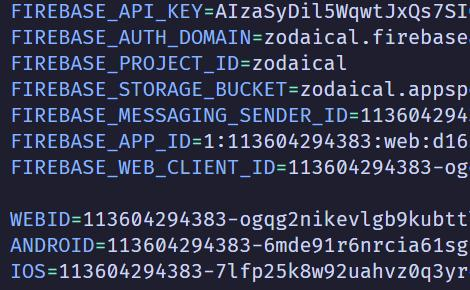
\includegraphics[height=6cm]{images/bezpieczenstwo/env}
	\caption{Zawartość pliku .env}
	\label{fig:Env}
\end{figure}

\newpage
W przypadku projektu ZodiaCal skorzystano ze zmiennych środowiskowych w pliku konfiguracyjnym Firebase, w plikach konfiguracyjnych do integracji zewnętrznych API obsługujących horoskop oraz bazę danych kosmetyków, w pliku SignIn ukrywając ID klienta potrzebnego do logowania się za pomocą konta Google oraz w miejscach w których skorzystano ze zdjęć z Firebase Storage (Rys.\ref{fig:FirebaseConfig}).

\begin{figure}[ht]
	\centering
	\vspace{0.25cm}
	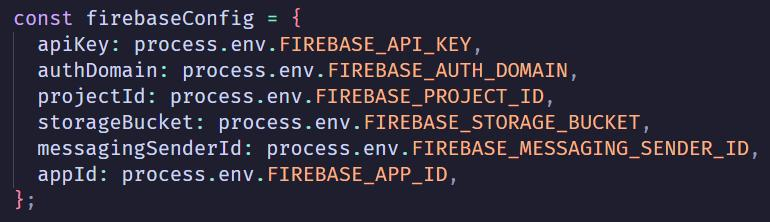
\includegraphics[height=4cm]{images/bezpieczenstwo/firebaseConfig}
	\caption{Wykorzystanie zmiennych globalnych w pliku konfiguracyjnym Firebase}
	\label{fig:FirebaseConfig}
\end{figure}

\section*{Walidacja formularzy}
\addcontentsline{toc}{section}{Walidacja formularzy}
Kluczowym sposobem na ochronę aplikacji przed atakami cybernetycznymi jest walidacja formularza. Pozwala ona na utrzymanie integralności danych i uniknięciu takich sytuacji, w których na przykład jeden użytkownik ma więcej, niż jedno konto przypisane do tego samego adresu e-mail. Można to osiągnąć korzystając z wbudowanych metod Firebase odwołując się do komunikatu błędu „auth/email-already-in-use” tak jak jest to widoczne na rysunku \ref{fig:Auth}.

\begin{figure}[ht]
	\centering
	\vspace{0.25cm}
	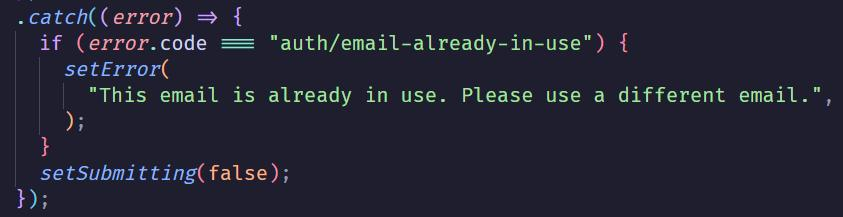
\includegraphics[height=4cm]{images/bezpieczenstwo/auth_email}
	\caption{Kod odpowiedzialny za weryfikację czy adres email jest już zapisany w bazie danych}
	\label{fig:Auth}
\end{figure}

Dodatkowo mechanizm wymuszający na klientach wprowadzenie silnego hasła, czyli takiego, które ma odpowiedną długość, posiada jedną wielką literę oraz znak specjalny, chroni konta użytkowników przed atakiem brute force polegającym na złamaniu hasła poprzez sprawdzanie przez algorytm wszystkich możliwych kombinacji tekstowych. Do weryfikacji, czy hasło zawiera specjalny znak skorzystano z wyrażenia regularnego, czyli ciągu znaków, który definiuje określony wzorzec.

\begin{figure}[ht]
	\centering
	\vspace{0.25cm}
	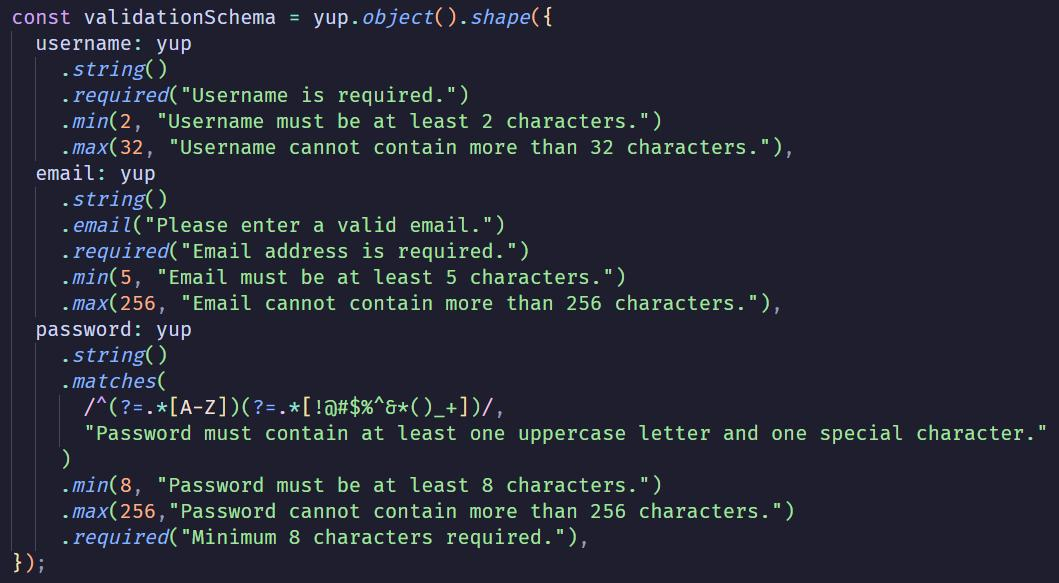
\includegraphics[height=8.5cm]{images/bezpieczenstwo/validationSchema}
	\caption{Kod odpowiedzialny za sprawdzenie siły hasła}
	\label{fig:Validation}
\end{figure}

W celu osiągnięcia wyżej wymienionych korzyści wykorzystano bibliotekę yup, która pozwala zdefiniować wymagania pól tekstowych w formularzu poprzez ustalenie typu zmiennej, określenie czy pole jest obowiązkowe oraz ustalenie długości ciągów znaków co przedstawiono na rysunku (Rys.\ref{fig:Validation}). Podane wartości maksymalne zostały zdefiniowane przez dokument RFC 5321 \cite{rfc} definiujący standardy dotyczące protokołu używanego do przekazywania wiadomości e-mail. Ustalenie limitów pól formularza jest kluczowe, aby zapobiec problemom związanych z wydajnością systemu.

Dodatkowo każdy warunek powinien mieć unikalny komunikat błędu. Jest to korzystne zarówno dla dewelopera jak i użytkownika, ponieważ można określić w którym momencie pojawił się problem.


\section*{Ograniczona liczba prób logowania}
\addcontentsline{toc}{section}{Ograniczona liczba prób logowania}
Kolejnym sposobem na zapewnienie bezpieczeństwa aplikacji jest kontrola liczby prób logowania się do systemu. Kod na rysunku \ref{fig:LiczbaProb} zwiększa licznik prób logowania wykorzystując funkcję do aktualizacji stanu.

\begin{figure}[ht]
	\centering
	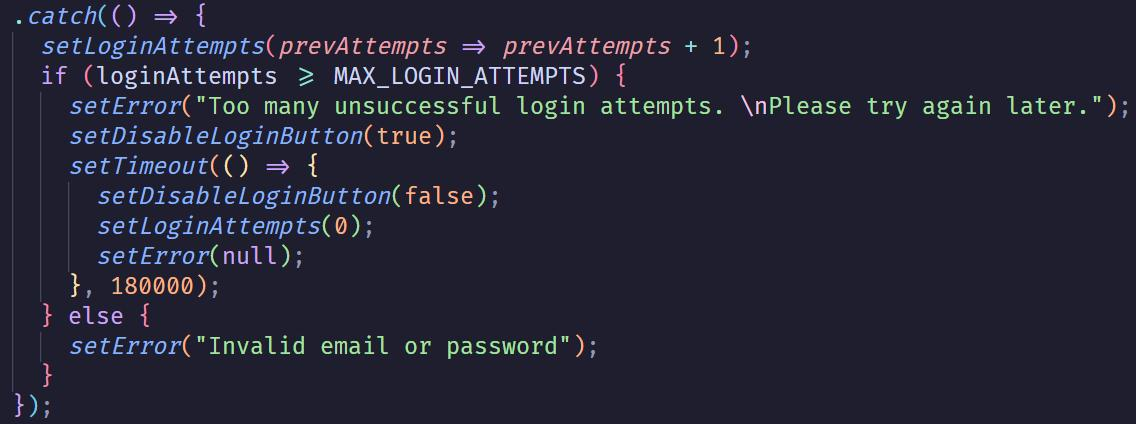
\includegraphics[height=5.6cm]{images/bezpieczenstwo/liczba_prob_kod}
	\caption{Fragment kodu odpowiadający za mechanizm zliczania prób logowania}
	\label{fig:LiczbaProb}
\end{figure}

 Następnie sprawdza, czy liczba prób przekracza wymaganą wartość. Jeśli tak, na ekranie pojawi się komunikat błędu, a przycisk logowania zostanie dezaktywowany (Rys.\ref{fig:Blad}). Użytkownik musi odczekać 3 minuty, po tym czasie licznik prób jest zerowany i można spróbować się zalogować.
\begin{figure}[H]
	\centering
	\vspace{0.25cm}
	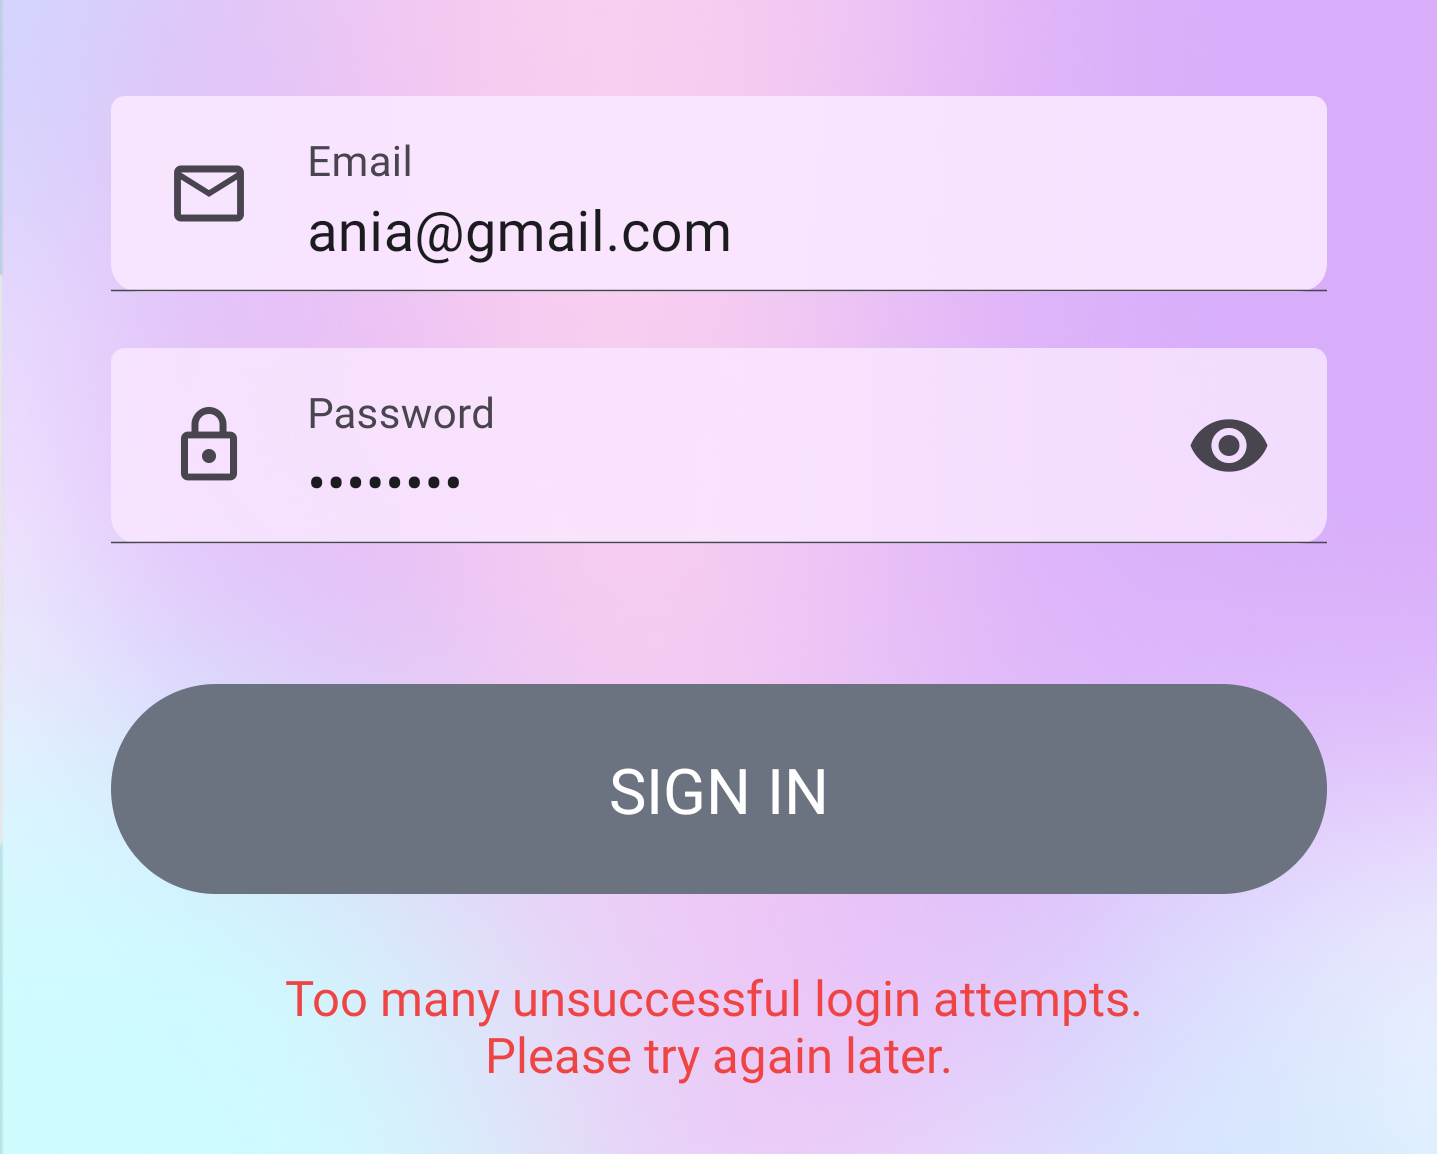
\includegraphics[height=5.7cm]{images/bezpieczenstwo/blad}
	\caption{Komunikat błędu informujący o błędnym wprowadzeniu hasła}
	\label{fig:Blad}
\end{figure}


\section*{Zarządzanie sesją użytkownika}
\addcontentsline{toc}{section}{Zarządzanie sesją użytkownika}
Po uzupełnieniu pól tekstowych formularza i wciśnięciu przycisku logowania, dane są weryfikowane za pomocą metody signInWithEmailAndPassword dostarczonej przez Firebase. Jeśli zostały poprawnie wprowadzone użytkownik zmieni stan i zostaje przeniesiony do głównej części aplikacji.

Zarządzanie sesją użytkownika chroni przed nieautoryzowanym dostępem do ukrytych zasobów aplikacji. Początkowo niezalogowany użytkownik ma dostęp jedynie do dwóch ekranów: SignIn oraz SignUp, natomiast po poprawnym zalogowaniu
i uwierzytelnieniu ma on dostęp do pełnej zawartości aplikacji.

Poniższy fragment kodu na rysunku \ref{fig:Nawigator} przedstawia nawigator, pełniący rolę kontrolera, który weryfikuje status zalogowania użytkownika i w oparciu o tę informację przenosi go między ekranami.
\\
\begin{figure}[ht]
	\centering
	\vspace{0.25cm}
	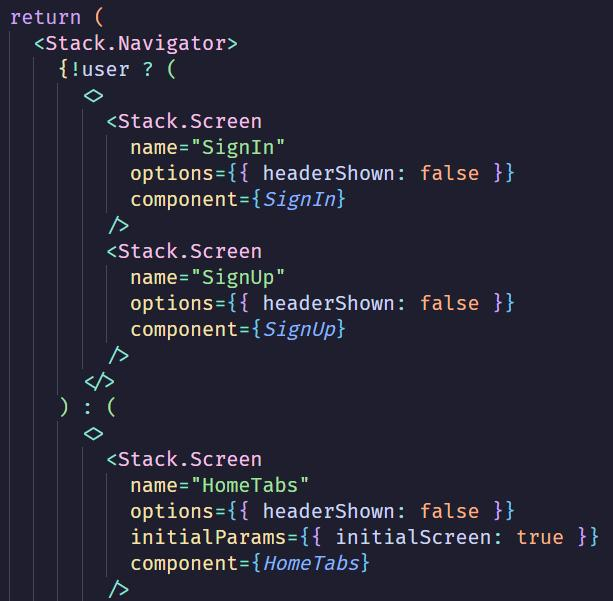
\includegraphics[height=12.22cm]{images/bezpieczenstwo/nawigator}
	\caption{Kod definiujący nawigację w zależności od stanu użytkownika}
	\label{fig:Nawigator}
\end{figure}


\section*{Archiwizacja}
\addcontentsline{toc}{section}{Archiwizacja}
Firebase zapewnia archiwizację bazy danych. Posiada narzędzia pozwalające na ręczne tworzenie kopii zapasowych oraz dodatkowo w płatnym planie Firebase cyklicznie, automatycznie tworzy kopie zapasowe. W przypadku aplikacji ZodiaCal kopia zapasowa bazy danych jest tworzone raz na miesiąc. Ta częstotliwość została ustalona na podstawie domyślnej konfiguracji Firebase oraz ograniczonych zasobów projektu.
Regularne kopie zapasowy usprawniają przywrócenie danych w przypadku ataku ransomware, polegającego na umyślnym zaszyfrowaniu lub uszkodzeniu bazy danych, w celu wymuszenia zapłaty okupu.



\chapter{Zakończenie}
Zakończenie pracy powinno zawierać ustosunkowanie się Autora do zadań wskazanych we Wstępie, a w szczególności do celu, miar i zakresu pracy oraz porównanie ich z faktycznymi wynikami pracy. Podejście takie umożliwia jasne określenie stopnia realizacji założonych celów oraz zwrócenie uwagi na wyniki osiągnięte przez Autora w ramach jego samodzielnej pracy. Ta część pracy powinna zawierać również omówienie trudności jakie wystąpiły przy realizacji pracy oraz zalet i wad przyjętego rozwiązania.


\printbibliography[heading=bibintoc, title={Bibliografia}]
\end{document}
